%
% ---------------------------------------------------------------
% Copyright (C) 2012-2018 Gang Li
% ---------------------------------------------------------------
%
% This work is the default powerdot-tuliplab style test file and may be
% distributed and/or modified under the conditions of the LaTeX Project Public
% License, either version 1.3 of this license or (at your option) any later
% version. The latest version of this license is in
% http://www.latex-project.org/lppl.txt and version 1.3 or later is part of all
% distributions of LaTeX version 2003/12/01 or later.
%
% This work has the LPPL maintenance status "maintained".
%
% This Current Maintainer of this work is Gang Li.
%
%

\documentclass[
 size=14pt,
 paper=smartboard,  %a4paper, smartboard, screen
 mode=present, 		%present, handout, print
 display=slides, 	% slidesnotes, notes, slides
 style=tuliplab,  	% TULIP Lab style
 pauseslide,
 fleqn,leqno]{powerdot}


\usepackage{cancel}
\usepackage{caption}
\usepackage{stackengine}
\usepackage{smartdiagram}
\usepackage{attrib}
\usepackage{amssymb}
\usepackage{amsmath} 
\usepackage{amsthm} 
\usepackage{mathtools}
\usepackage{rotating}
\usepackage{graphicx}
\usepackage{boxedminipage}
\usepackage{rotate}
\usepackage{calc}
\usepackage[absolute]{textpos}
\usepackage{psfrag,overpic}
\usepackage{fouriernc}
\usepackage{pstricks,pst-3d,pst-grad,pstricks-add,pst-text,pst-node,pst-tree}
\usepackage{moreverb,epsfig,subfigure}
\usepackage{color}
\usepackage{booktabs}
\usepackage{etex}
\usepackage{breqn}
\usepackage{multirow}
\usepackage{natbib}
\usepackage{bibentry}
\usepackage{gitinfo2}
\usepackage{siunitx}
\usepackage{nicefrac}
%\usepackage{geometry}
%\geometry{verbose,letterpaper}
\usepackage{media9}
\usepackage{animate}
%\usepackage{movie15}
\usepackage{auto-pst-pdf}

\usepackage{breakurl}
\usepackage{fontawesome}
\usepackage{xcolor}
\usepackage{multicol}



\usepackage{verbatim}
\usepackage[utf8]{inputenc}
\usepackage{C:/texlive/2022/dtk-logos}
\usepackage{tikz}
\usepackage{adigraph}
%\usepackage{tkz-graph}
\usepackage{hyperref}
%\usepackage{ulem}
\usepackage{pgfplots}
\usepackage{verbatim}
\usepackage{fontawesome}


\usepackage{todonotes}
% \usepackage{pst-rel-points}
\usepackage{animate}
\usepackage{fontawesome}

\usepackage{listings}
\lstset{frameround=fttt,
frame=trBL,
stringstyle=\ttfamily,
backgroundcolor=\color{yellow!20},
basicstyle=\footnotesize\ttfamily}
\lstnewenvironment{code}{
\lstset{frame=single,escapeinside=`',
backgroundcolor=\color{yellow!20},
basicstyle=\footnotesize\ttfamily}
}{}


\usepackage{hyperref}
\hypersetup{ % TODO: PDF meta Data
  pdftitle={Air Pollution Measurements Prediction},
  pdfauthor={Yu Li},
  pdfpagemode={FullScreen},
  pdfborder={0 0 0}
}


% \usepackage{auto-pst-pdf}
% package to show source code

\definecolor{LightGray}{rgb}{0.9,0.9,0.9}
\newlength{\pixel}\setlength\pixel{0.000714285714\slidewidth}
\setlength{\TPHorizModule}{\slidewidth}
\setlength{\TPVertModule}{\slideheight}
\newcommand\highlight[1]{\fbox{#1}}
\newcommand\icite[1]{{\footnotesize [#1]}}

\newcommand\twotonebox[2]{\fcolorbox{pdcolor2}{pdcolor2}
{#1\vphantom{#2}}\fcolorbox{pdcolor2}{white}{#2\vphantom{#1}}}
\newcommand\twotoneboxo[2]{\fcolorbox{pdcolor2}{pdcolor2}
{#1}\fcolorbox{pdcolor2}{white}{#2}}
\newcommand\vpspace[1]{\vphantom{\vspace{#1}}}
\newcommand\hpspace[1]{\hphantom{\hspace{#1}}}
\newcommand\COMMENT[1]{}

\newcommand\placepos[3]{\hbox to\z@{\kern#1
        \raisebox{-#2}[\z@][\z@]{#3}\hss}\ignorespaces}

\renewcommand{\baselinestretch}{1.2}


\newcommand{\draftnote}[3]{
	\todo[author=#2,color=#1!30,size=\footnotesize]{\textsf{#3}}	}
% TODO: add yourself here:
%
\newcommand{\gangli}[1]{\draftnote{blue}{GLi:}{#1}}
\newcommand{\shaoni}[1]{\draftnote{green}{sn:}{#1}}
\newcommand{\gliMarker}
	{\todo[author=GLi,size=\tiny,inline,color=blue!40]
	{Gang Li has worked up to here.}}
\newcommand{\snMarker}
	{\todo[author=Sn,size=\tiny,inline,color=green!40]
	{Shaoni has worked up to here.}}

%%%%%%%%%%%%%%%%%%%%%%%%%%%%%%%%%%%%%%%%%%%%%%%%%%%%%%%%%%%%%%%%%%%%%%%%
% title
% TODO: Customize to your Own Title, Name, Address
%
\title{Air Pollution Measurements Prediction}
\author{
Yu Li
\\
\\Nanjing University of Science and Technology
\\Deakin University
\\Chinese Academy of Sciences
}
\date{\gitCommitterDate}


% Customize the setting of slides
\pdsetup{
% TODO: Customize the left footer, and right footer
rf=\href{http://www.tulip.org.au}{
Last Changed by: \textsc{\gitCommitterName}\ \gitVtagn-\gitAbbrevHash\ (\gitAuthorDate)
},
cf={Air Pollution Measurements Prediction},
}


\begin{document}

\maketitle

%\begin{slide}{Overview}
%\tableofcontents[content=sections]
%\end{slide}


%%==========================================================================================
%%
\begin{slide}[toc=,bm=]{Overview}
\tableofcontents[content=currentsection,type=1]
\end{slide}
%%
%%==========================================================================================


\section{Problem Definition}


%%==========================================================================================
%%
\begin{slide}{Air Pollution Measurements Prediction}
\begin{center}
\twotonebox{\rotatebox{90}{}}{\parbox{.86\textwidth}
{In this competition you are predicting the values of air pollution measurements over time, 
	based on basic weather information \textcolor{orange}{(temperature and humidity)} and the input values of \textcolor{orange}{5 sensors}.
	The three target values to you to predict are:
\begin{itemize}
\item target_carbon_monoxide
\item target_benzene
\item target_nitrogen_oxides
\end{itemize}
}}
\end{center}
\end{slide}
%%
%%==========================================================================================


\section{Data Description}


%%==========================================================================================
%%
\begin{slide}{Train Data Description}
	\begin{center}
		\begin{tabular}{c| c }
			\toprule
			%\centering
			Elements & \texttt{Number}  \\
			\midrule
			$date time$
			&  {$7111$} \\
			$deg C$
			&  {$408$} \\
			$relative humidity$
			&  {$762$}  \\
			$absolute humidity$
			&  {$5451$}  \\
			$sensor 1$
			&  {$3882$} \\
			$sensor 2$
			&  {$3882$} \\
			$sensor 3$
			&  {$3882$} \\
			$sensor 4$
			&  {$3882$} \\
			$sensor 5$
			&  {$3882$} \\
			$target carbon monoxide$
			&  {$95$} \\
			$target benzene$
			&  {$405$} \\
			$target nitrogen oxides$
			&  {$3268$} \\
			\bottomrule
		\end{tabular}
	\end{center}
\end{slide}
%%
%%==========================================================================================

%%==========================================================================================
%%
\begin{slide}{Test Data Description}
	\begin{center}
	\begin{tabular}{c| c }
		\toprule
		%\centering
		Elements & \texttt{Number}  \\
		\midrule
		$date time$
		&  {$2247$} \\
		$deg C$
		&  {$280$} \\
		$relative humidity$
		&  {$653$}  \\
		$absolute humidity$
		&  {$1915$}  \\
		$sensor 1$
		&  {$1758$} \\
		$sensor 2$
		&  {$1816$} \\
		$sensor 3$
		&  {$1833$} \\
		$sensor 4$
		&  {$1877$} \\
		$sensor 5$
		&  {$2017$} \\
		\bottomrule
	\end{tabular}
	\end{center}
\end{slide}
%%
%%==========================================================================================


%%==========================================================================================
%%
\begin{slide}[toc=,bm=]{Data Visualization}

\begin{figure}
  \centering
  \selectcolormodel{rgb}
  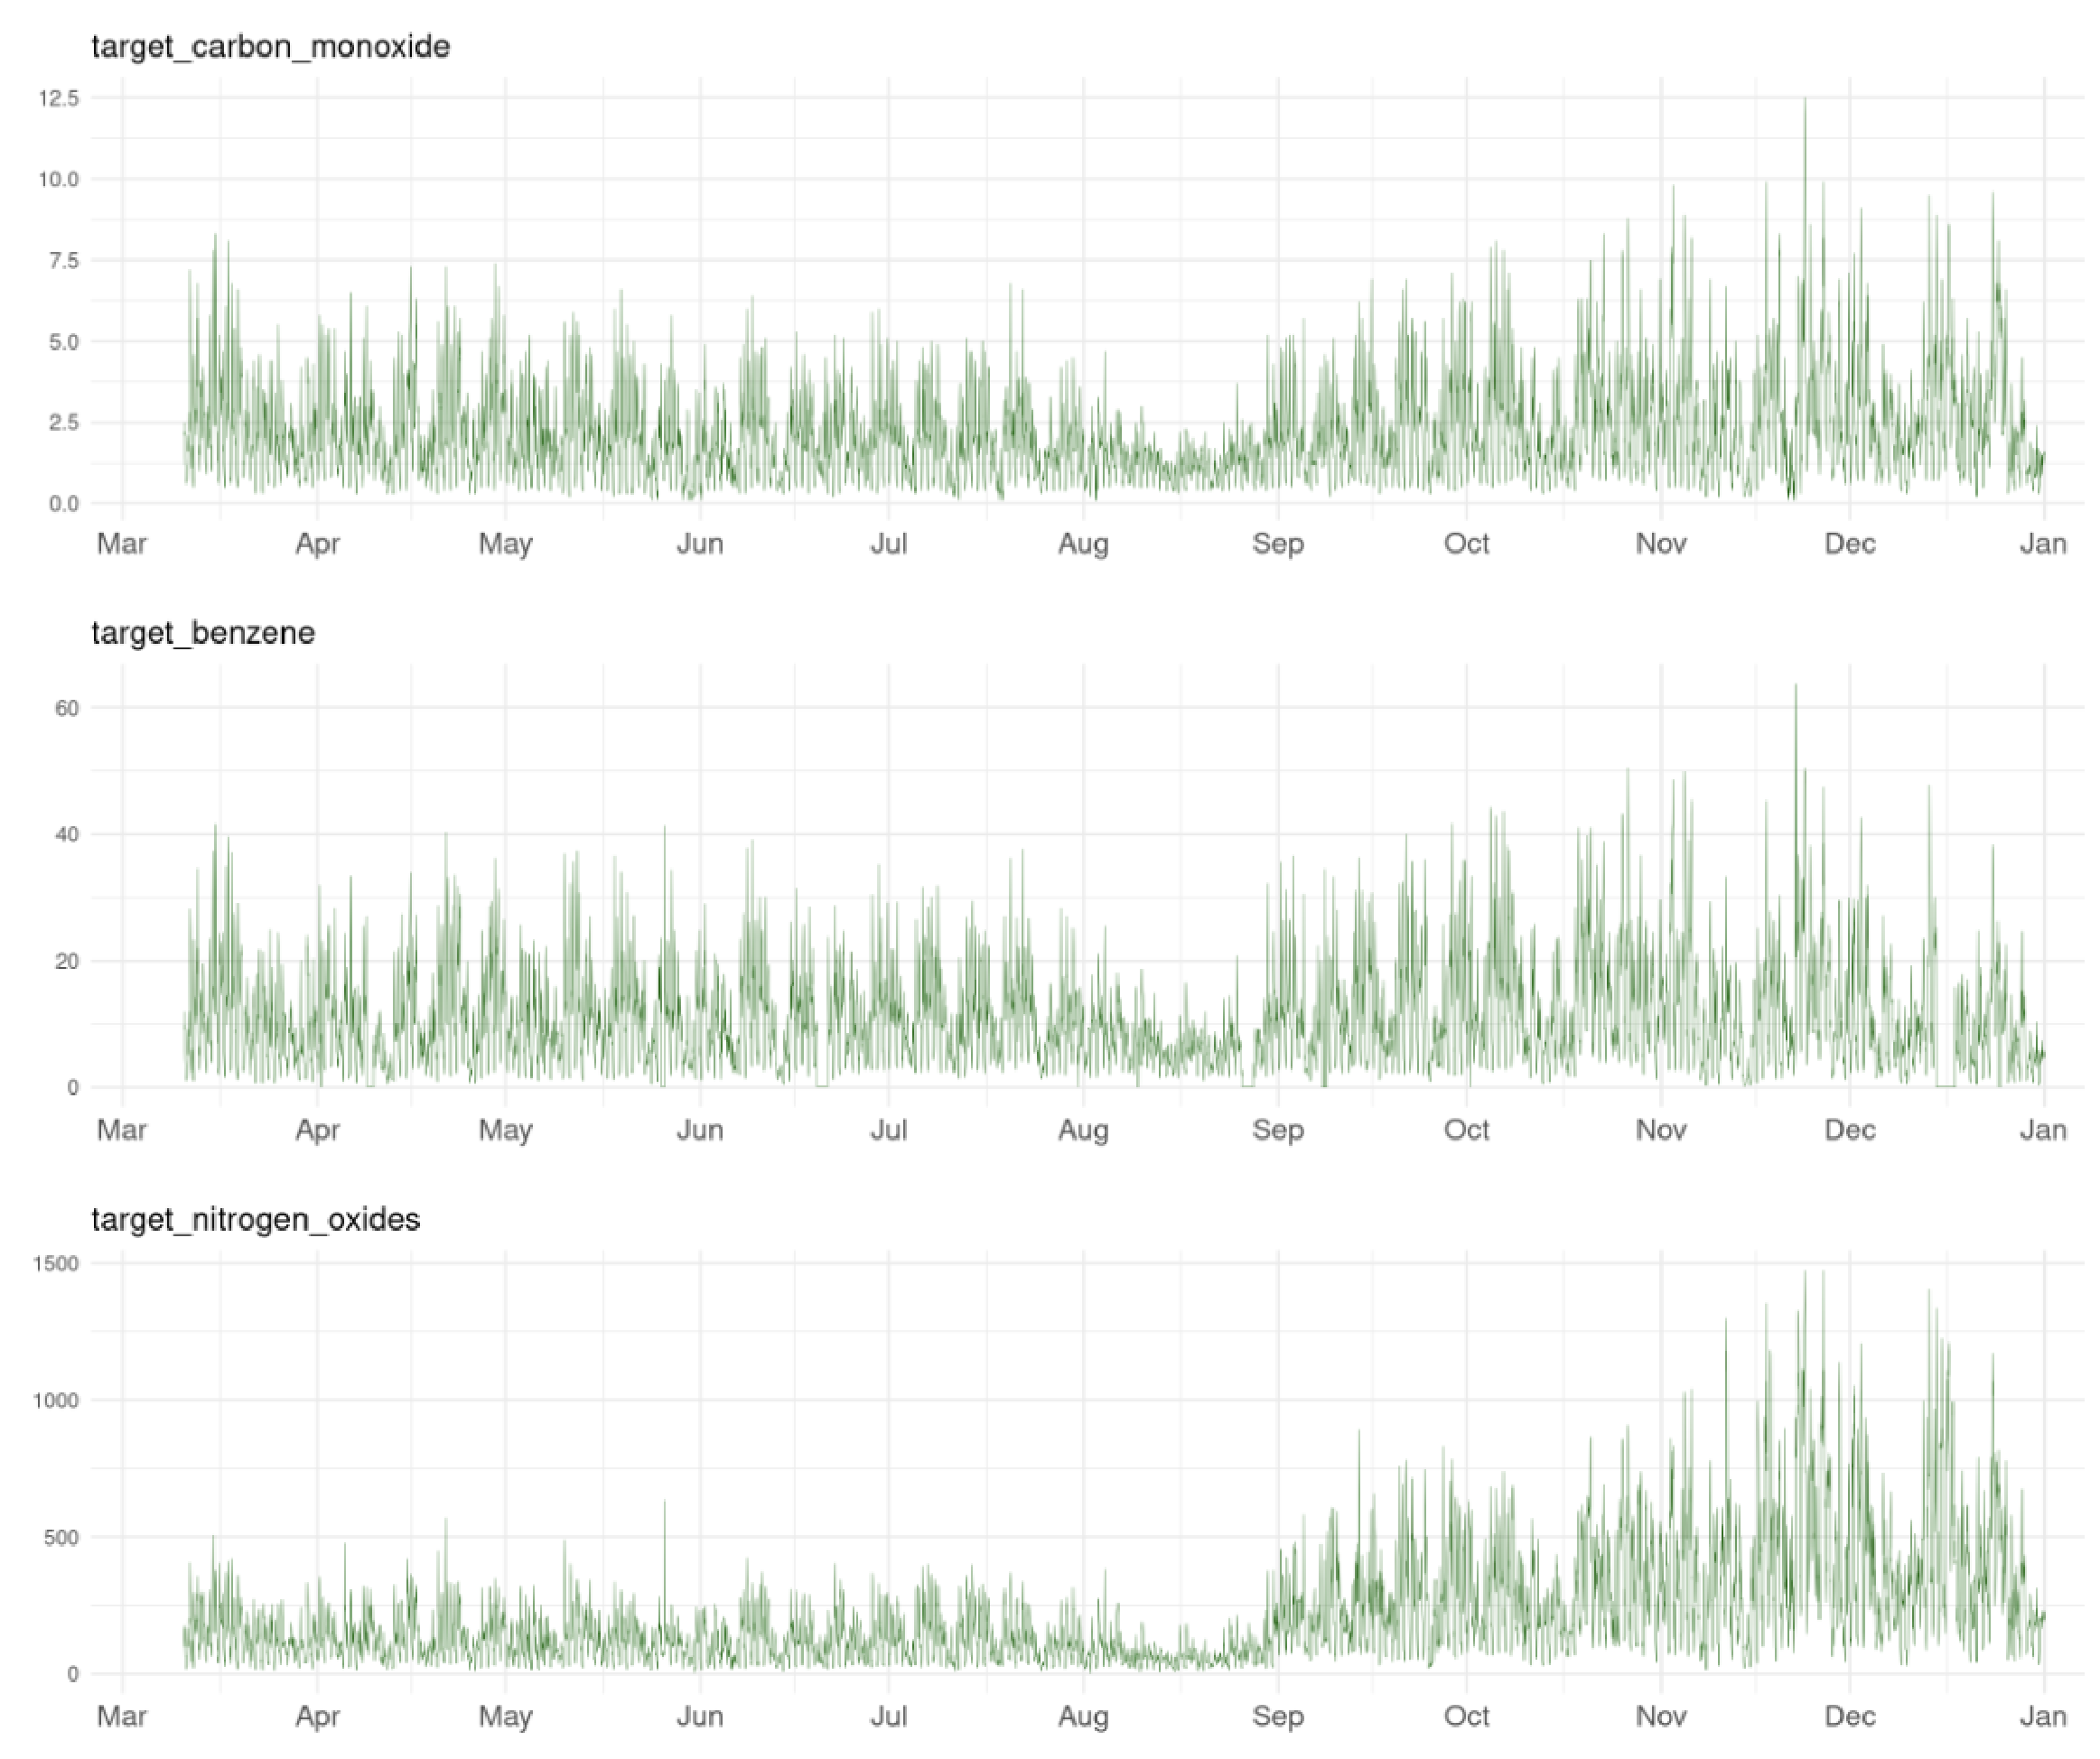
\includegraphics[scale=0.3]{figures//p1.eps}\\
  \caption{Target Overall Situation}\label{fig:Target Overall Situation}
\end{figure}

\end{slide}
%%
%%==========================================================================================

%%==========================================================================================
%%
\begin{slide}[toc=,bm=]{Data Visualization(2)}
	
	\begin{figure}
		\centering
		\selectcolormodel{rgb}
        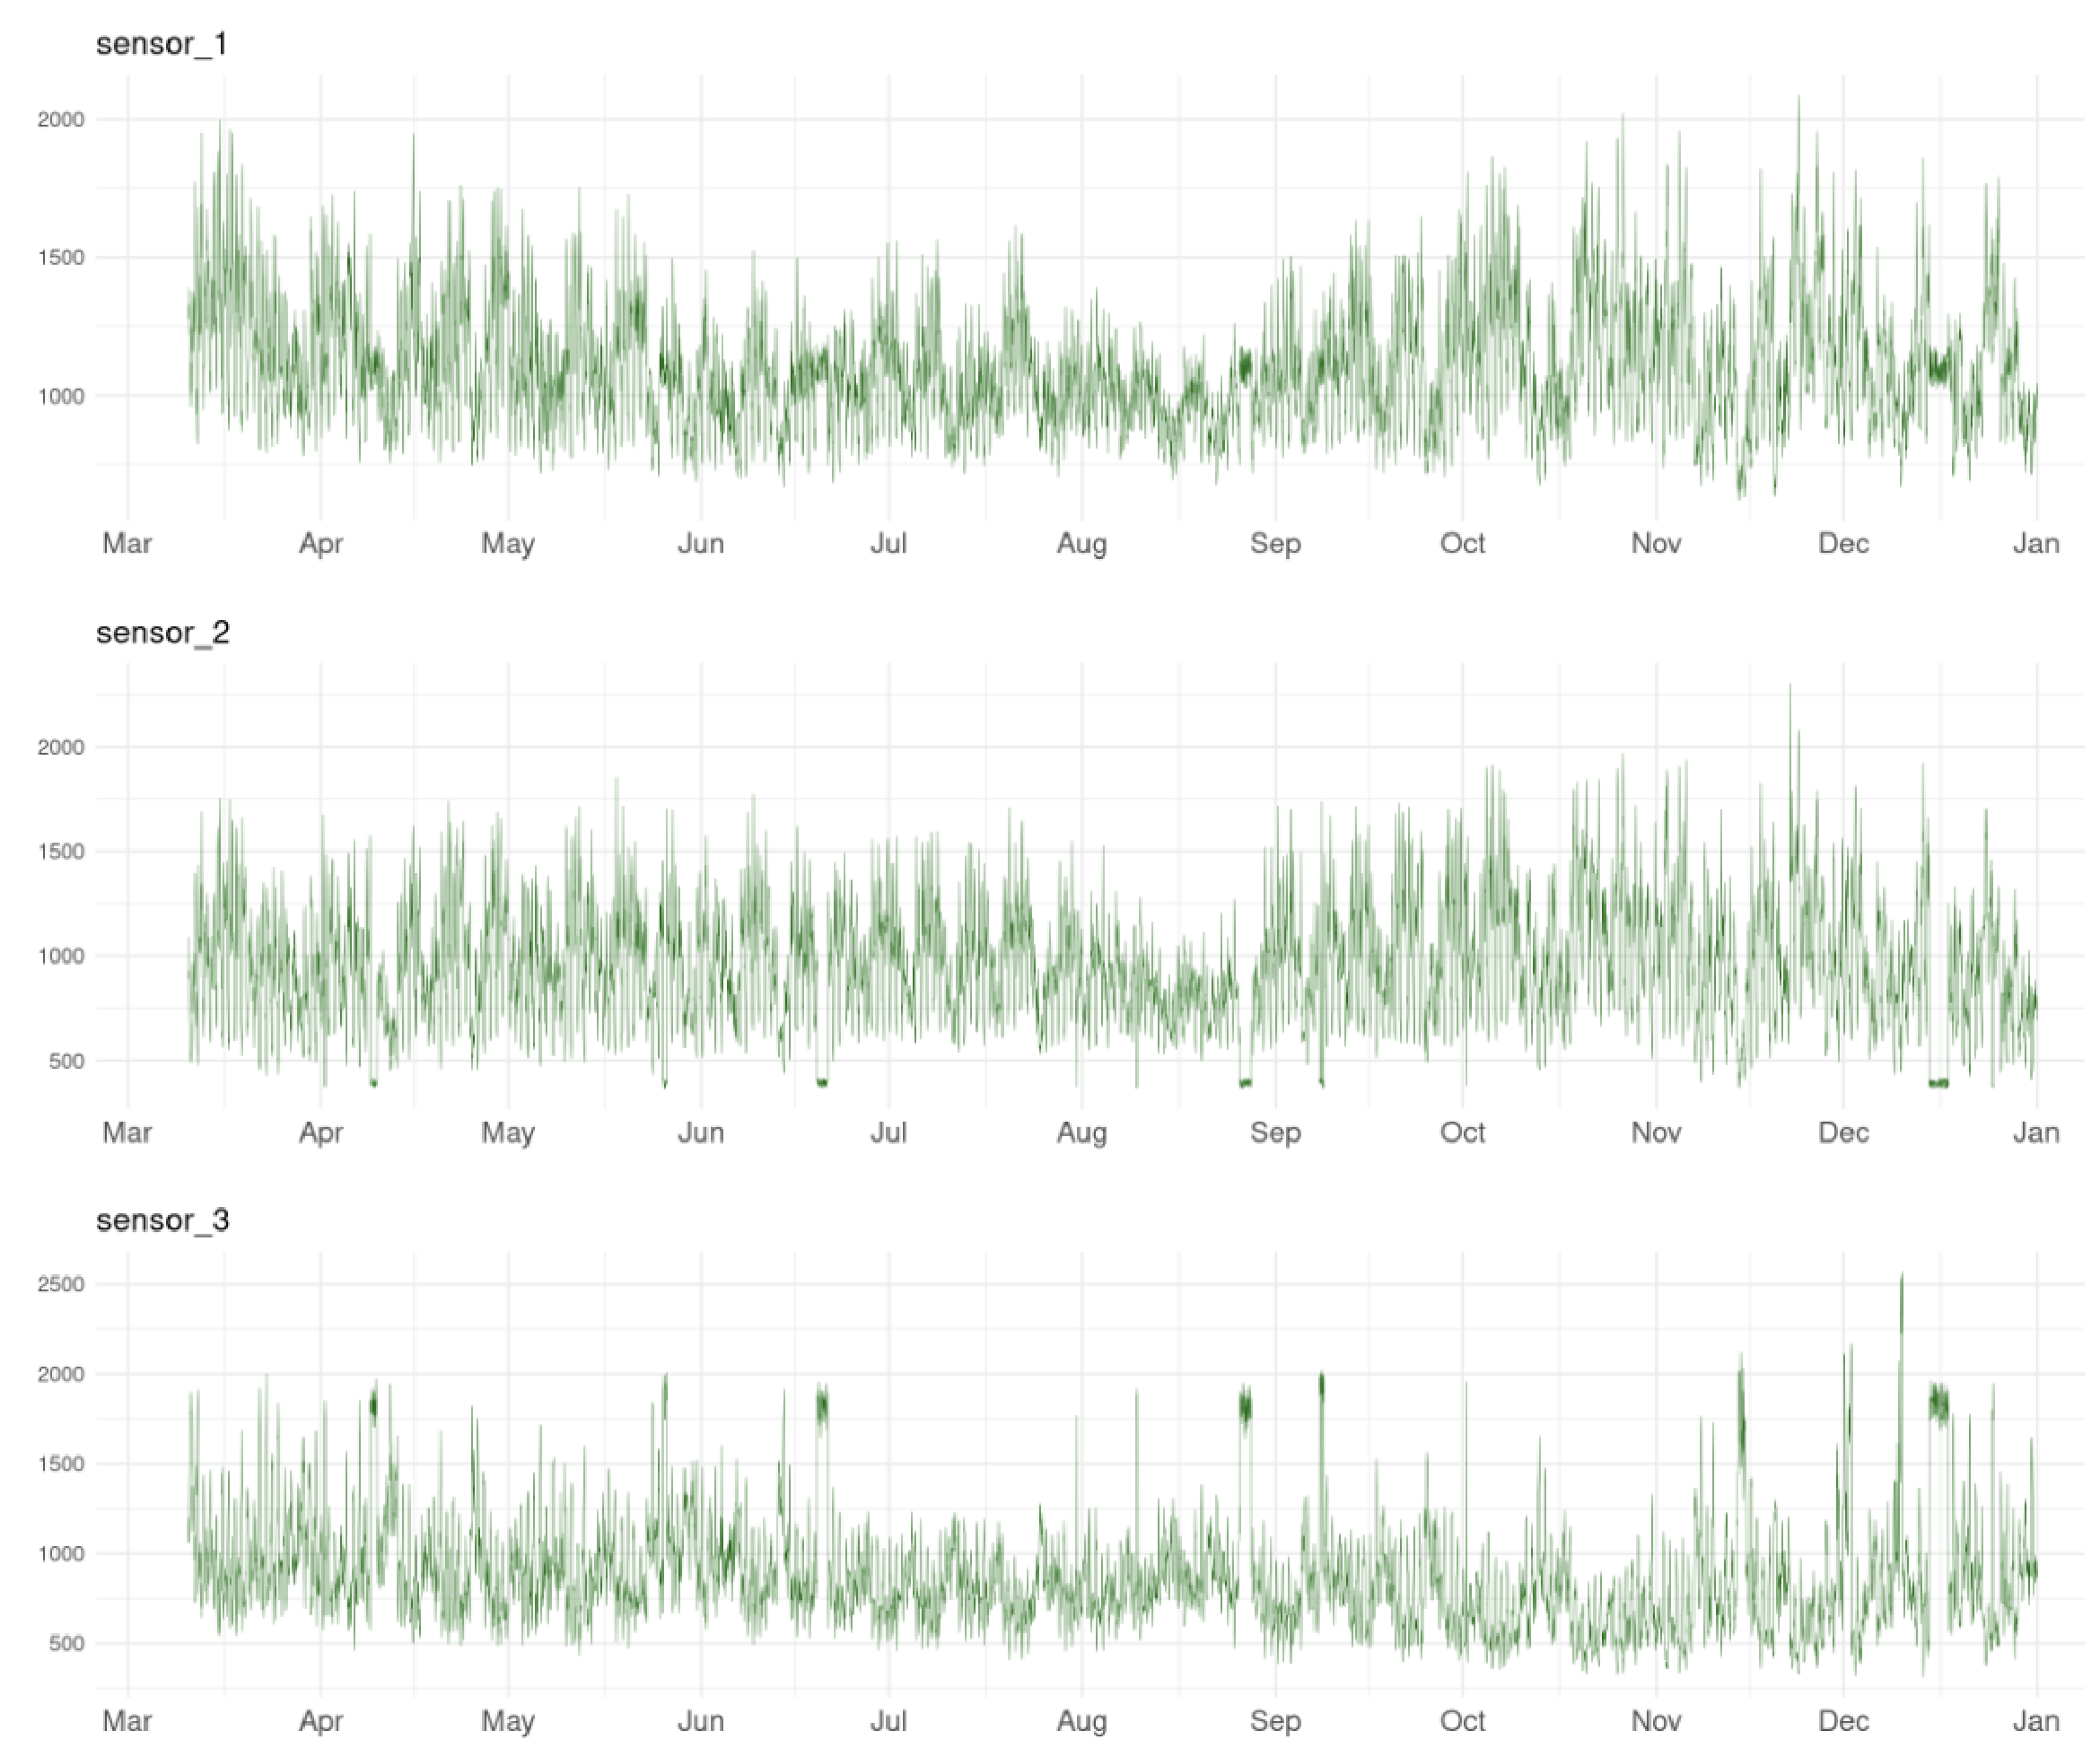
\includegraphics[scale=0.3]{figures//p2.eps}\\
		\caption{Sensor(1-3) Overall Situation}\label{fig:Sensor(1-3) Overall Situation}
	\end{figure}
	
\end{slide}
%%
%%==========================================================================================

%%==========================================================================================
%%
\begin{slide}[toc=,bm=]{Data Visualization(3)}
	
	\begin{figure}
		\centering
		\selectcolormodel{rgb}
        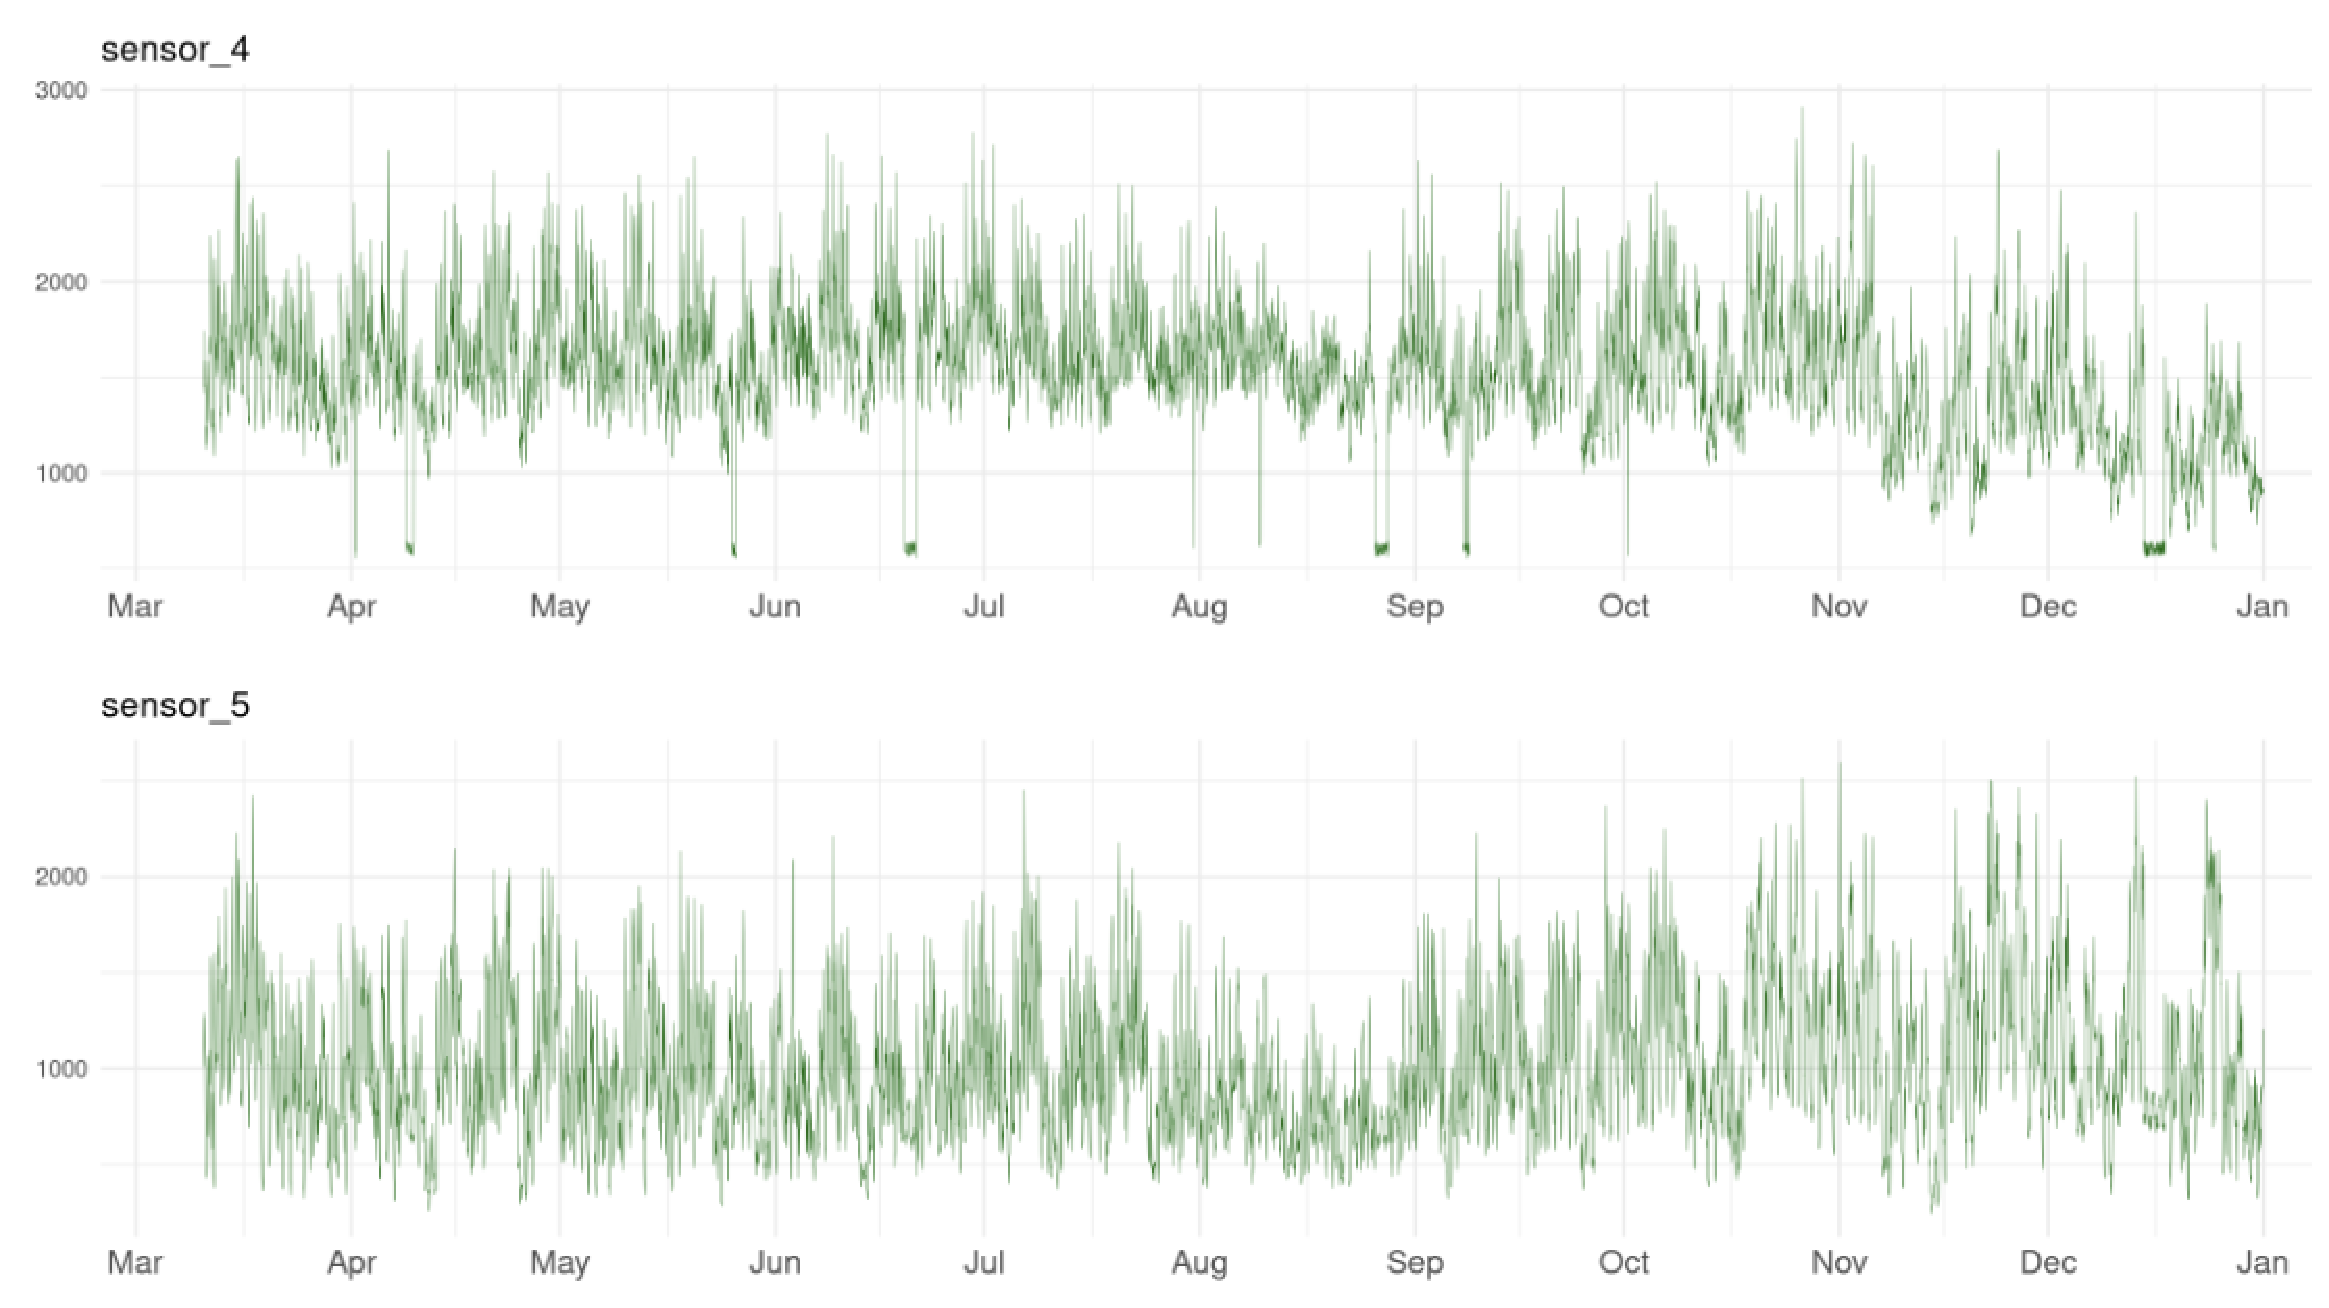
\includegraphics[scale=0.35]{figures//p3.eps}\\
		\caption{Sensor(4-5) Overall Situation}\label{fig:Sensor(4-5) Overall Situation}
	\end{figure}
	
\end{slide}
%%
%%==========================================================================================

%%==========================================================================================
%%
\begin{slide}[toc=,bm=]{Data Visualization(4)}
	
	\begin{figure}
		\centering
		\selectcolormodel{rgb}
        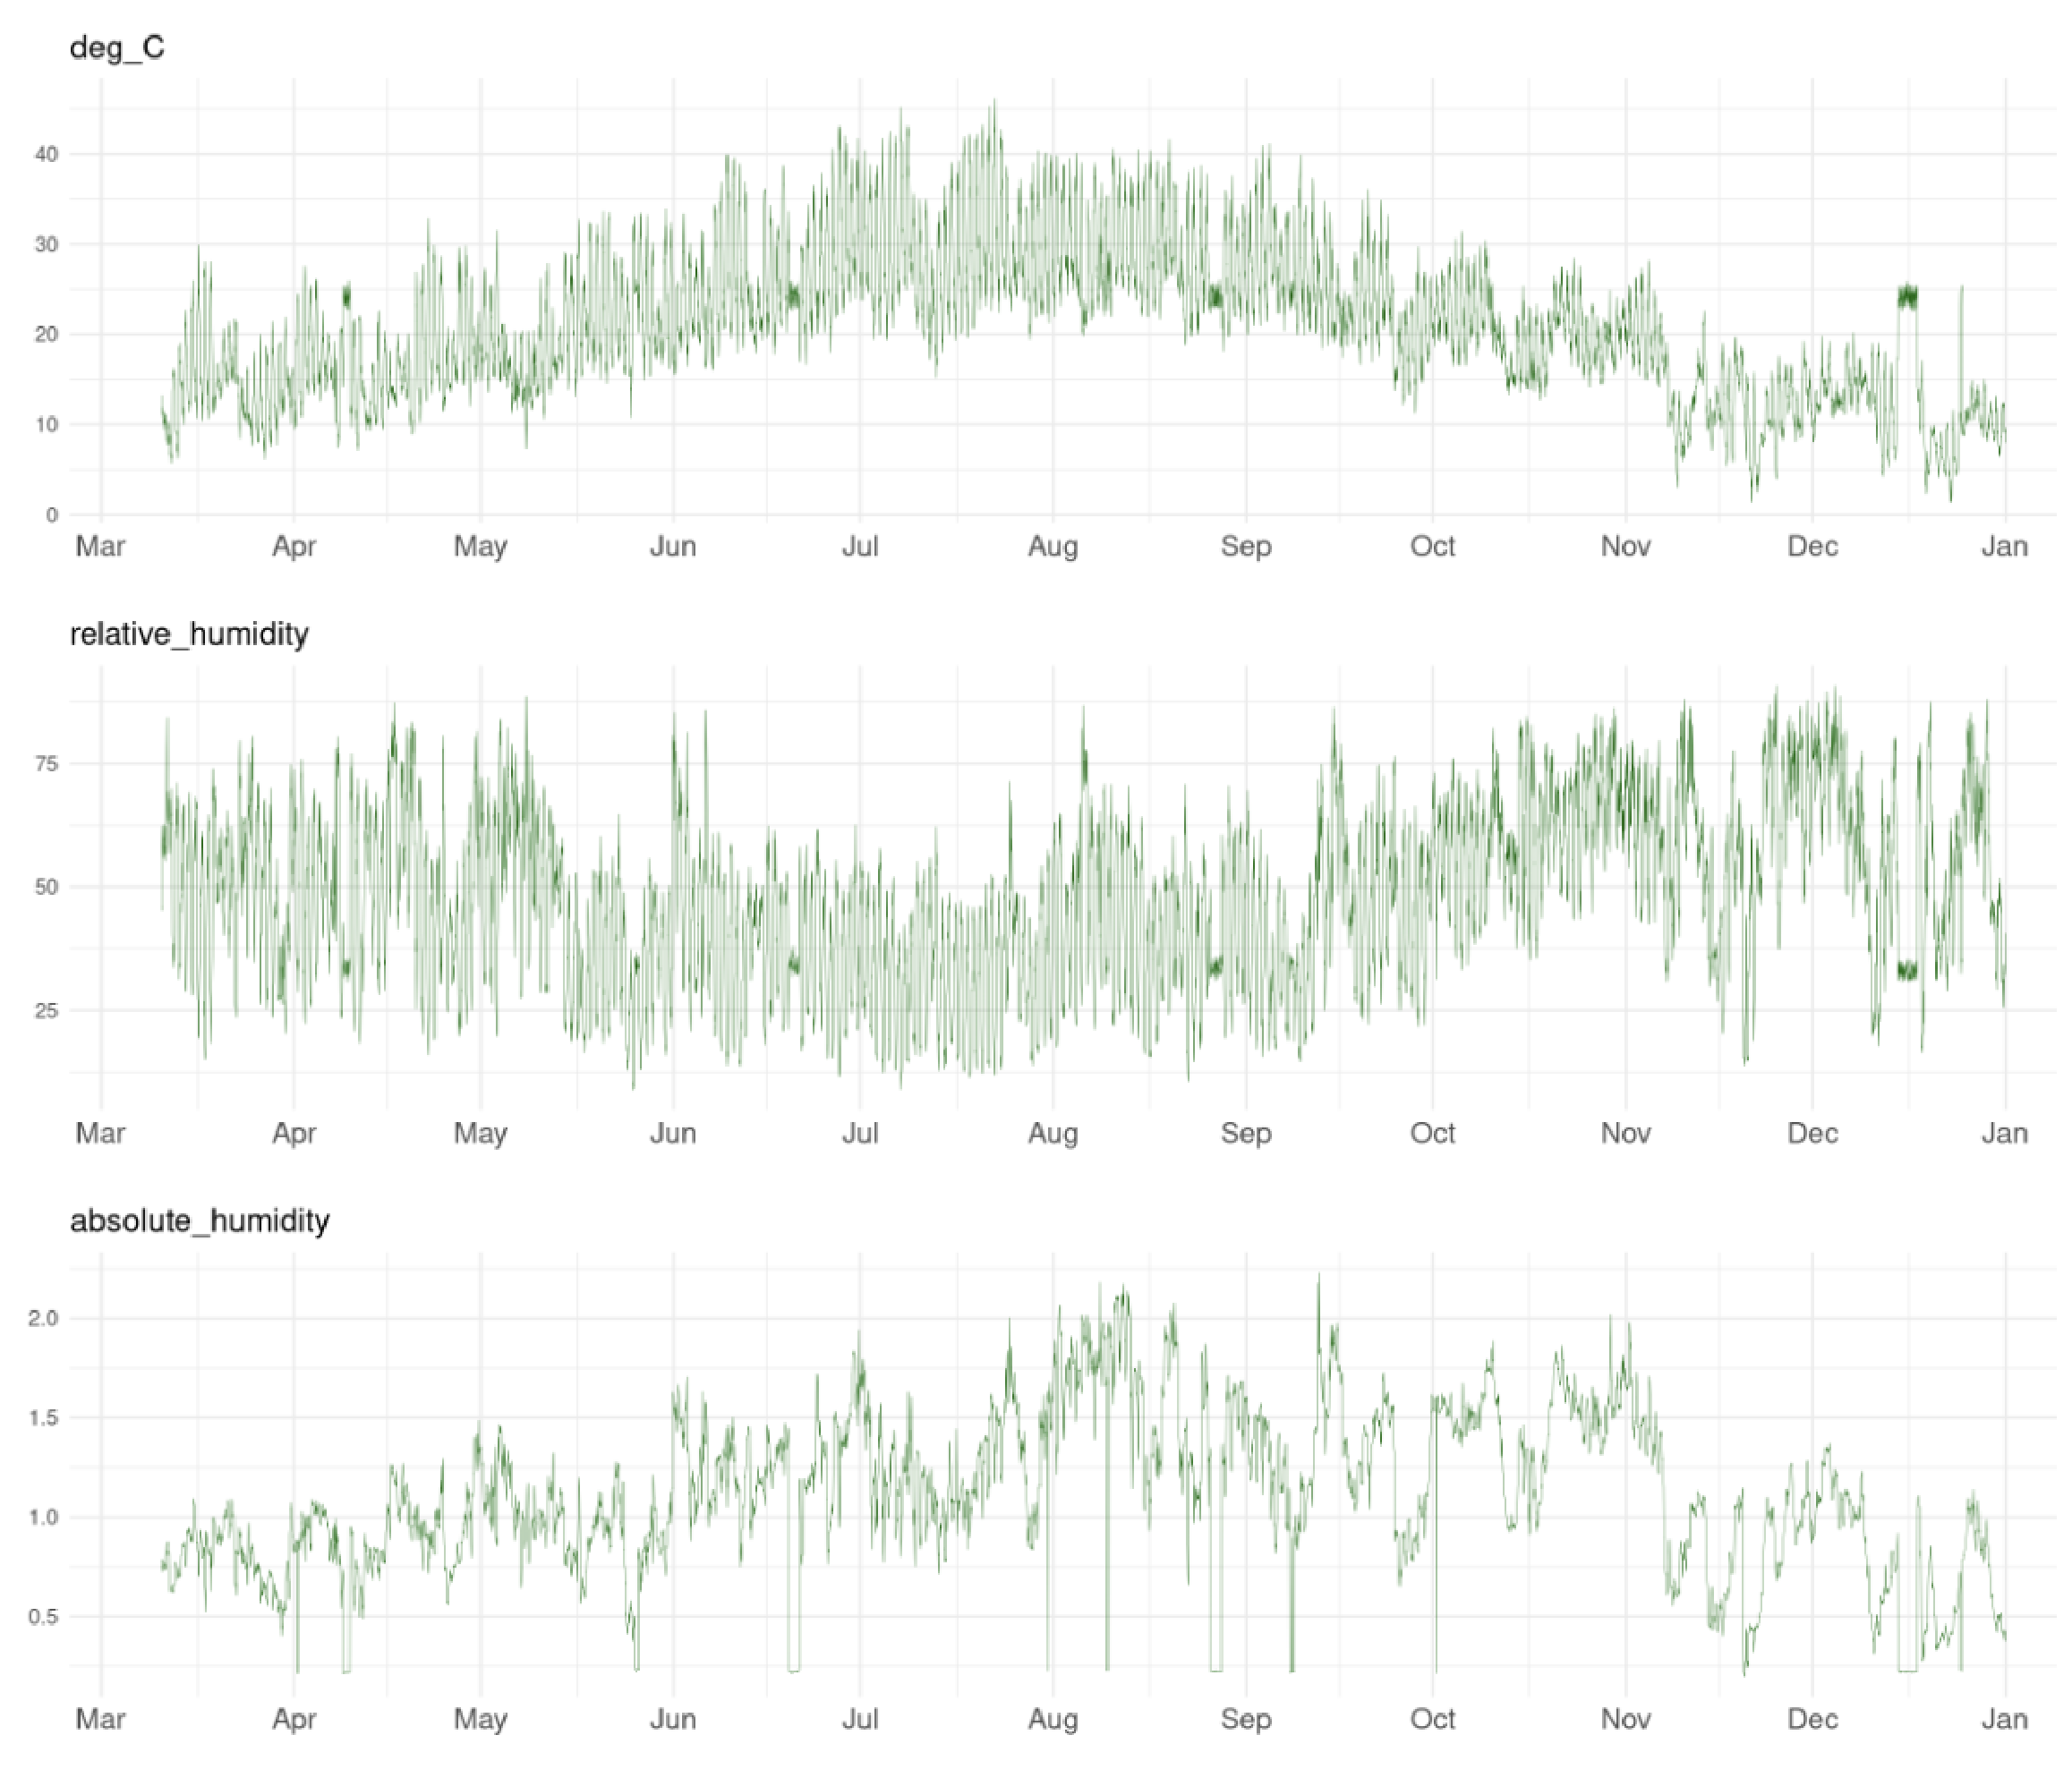
\includegraphics[scale=0.3]{figures//p4.eps}\\
		\caption{Weather Overall Situation}\label{fig:Weather Overall Situation}
	\end{figure}
	
\end{slide}
%%
%%==========================================================================================

%%==========================================================================================
%%
\begin{slide}[toc=,bm=]{Data Visualization(5)}
	
	\begin{figure}
		\centering
		\selectcolormodel{rgb}
        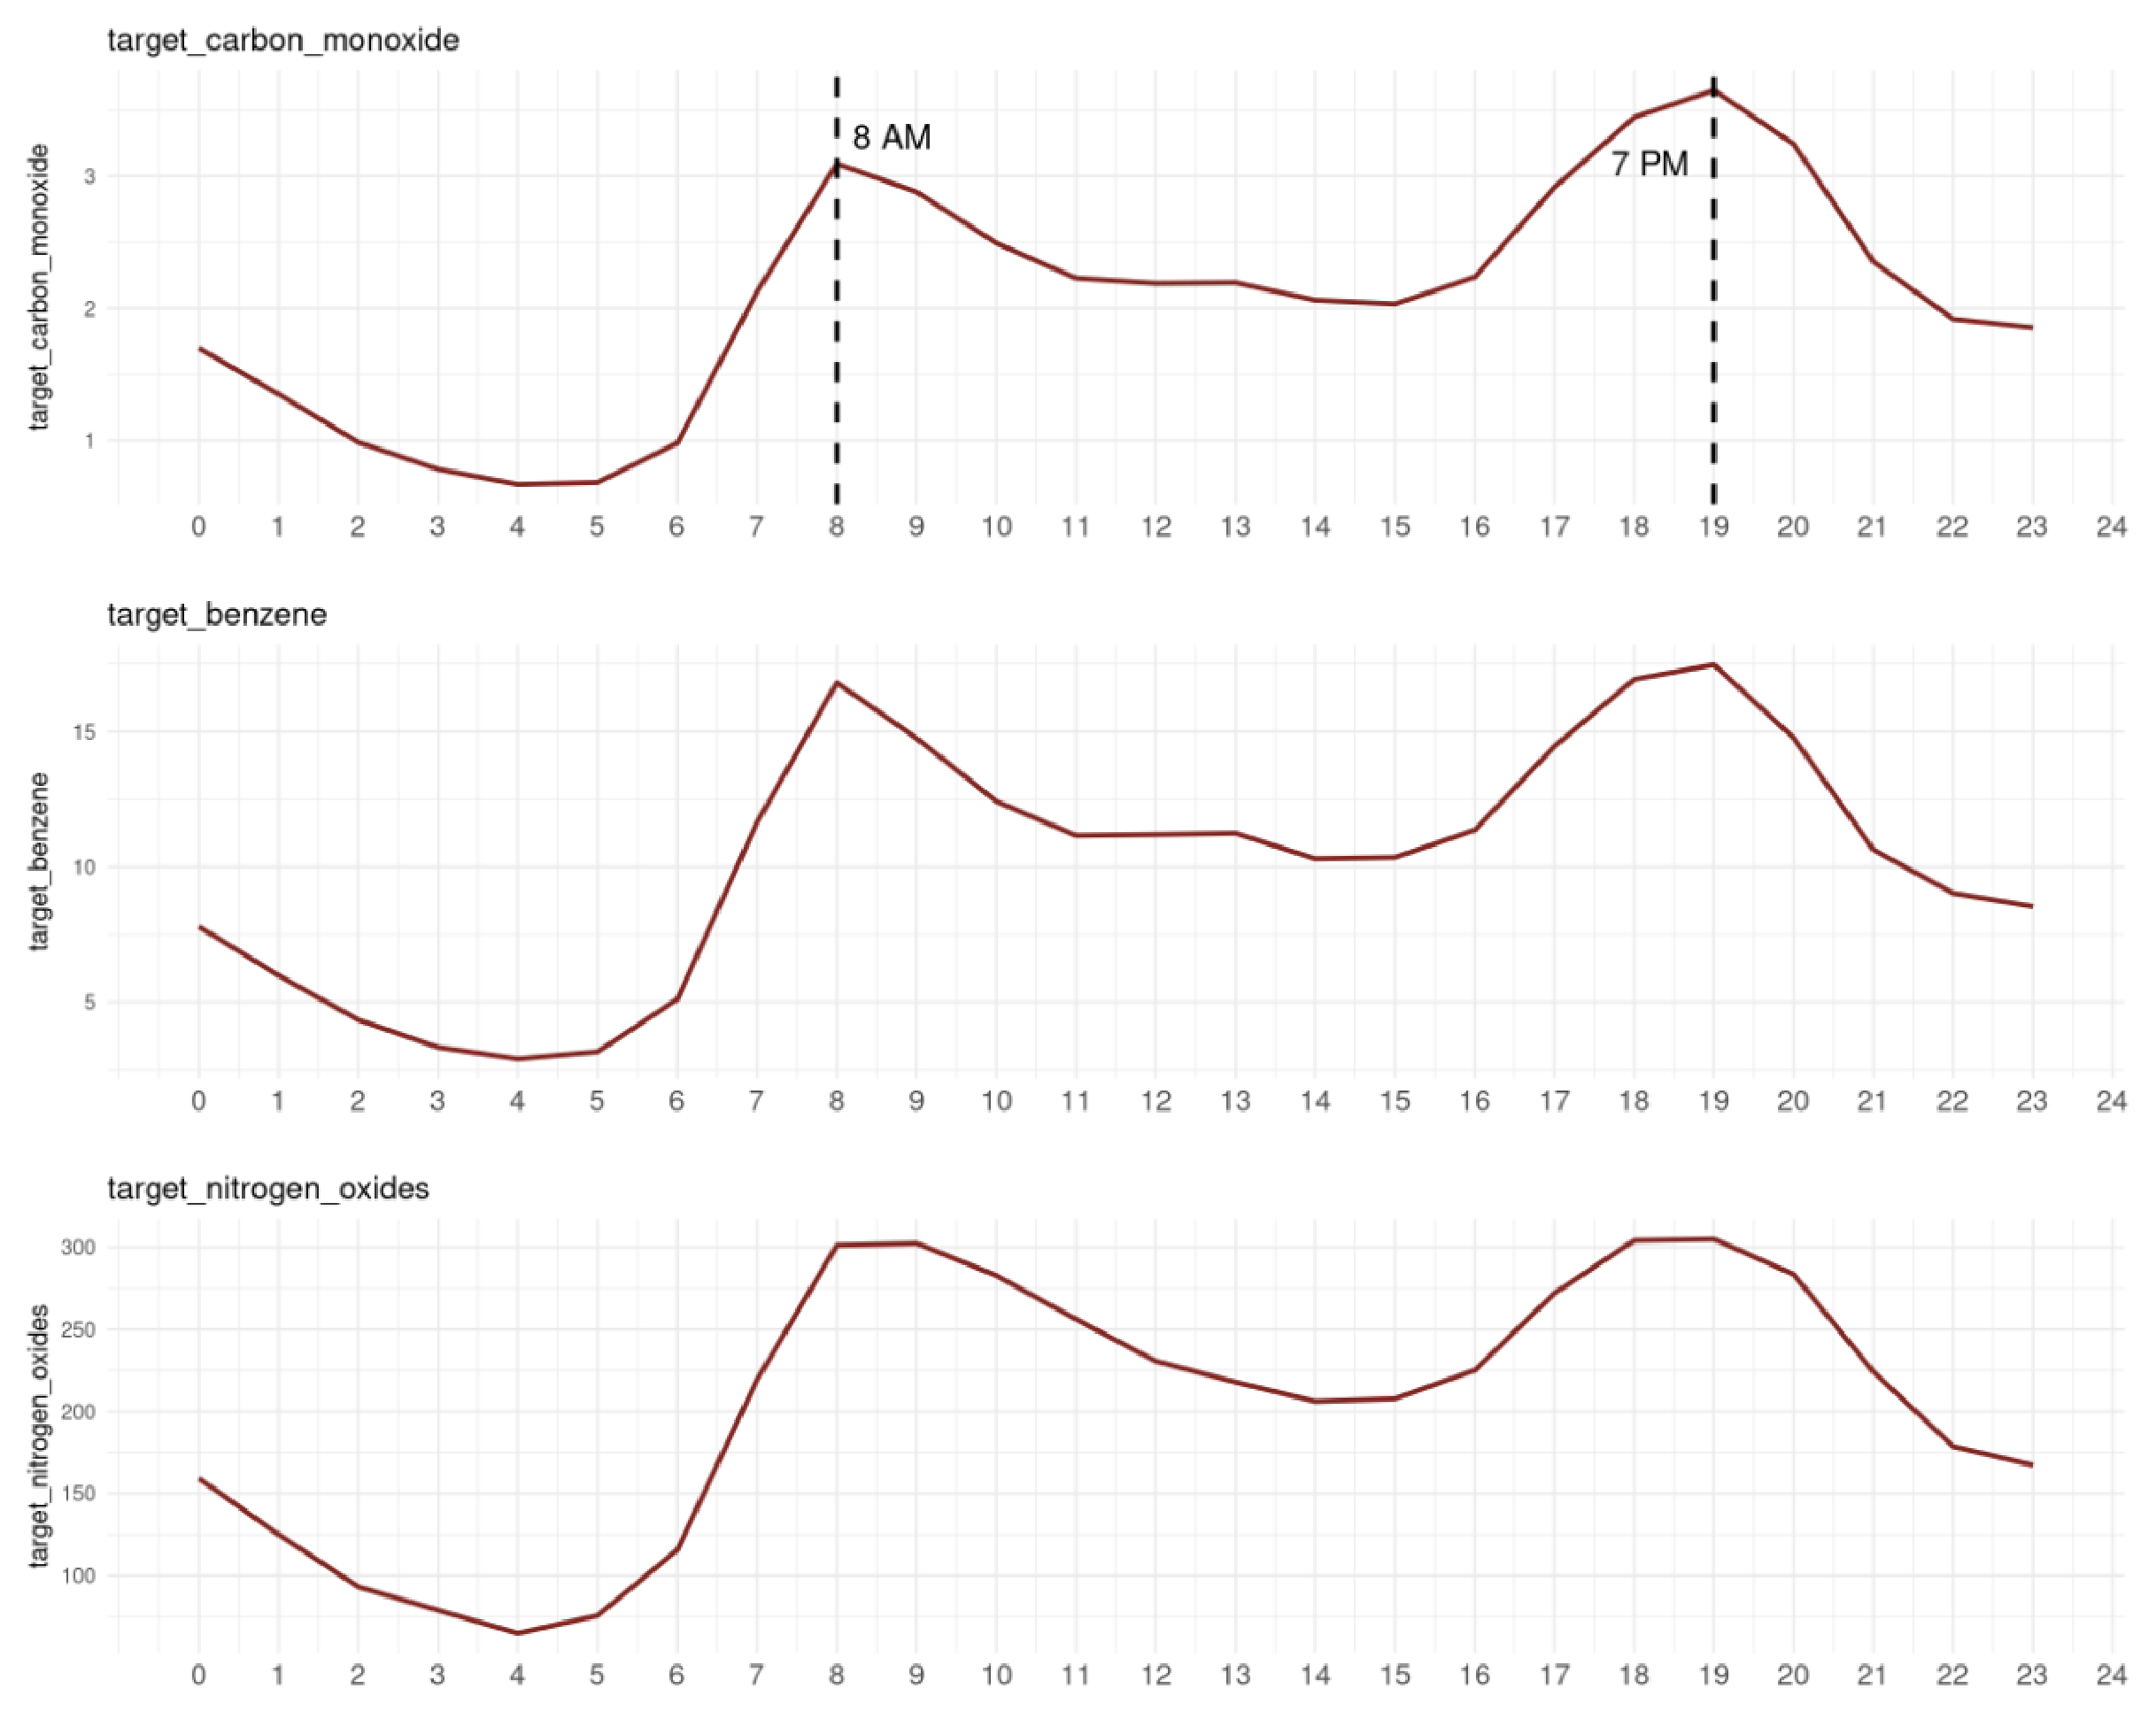
\includegraphics[scale=0.3]{figures//p5.eps}\\
		\caption{Target Daily Hourly Change}\label{fig:Target Daily Hourly Change}
	\end{figure}
	
\end{slide}
%%
%%==========================================================================================

%%==========================================================================================
%%
\begin{slide}[toc=,bm=]{Data Visualization(6)}
	
	\begin{figure}
		\centering
		\selectcolormodel{rgb}
        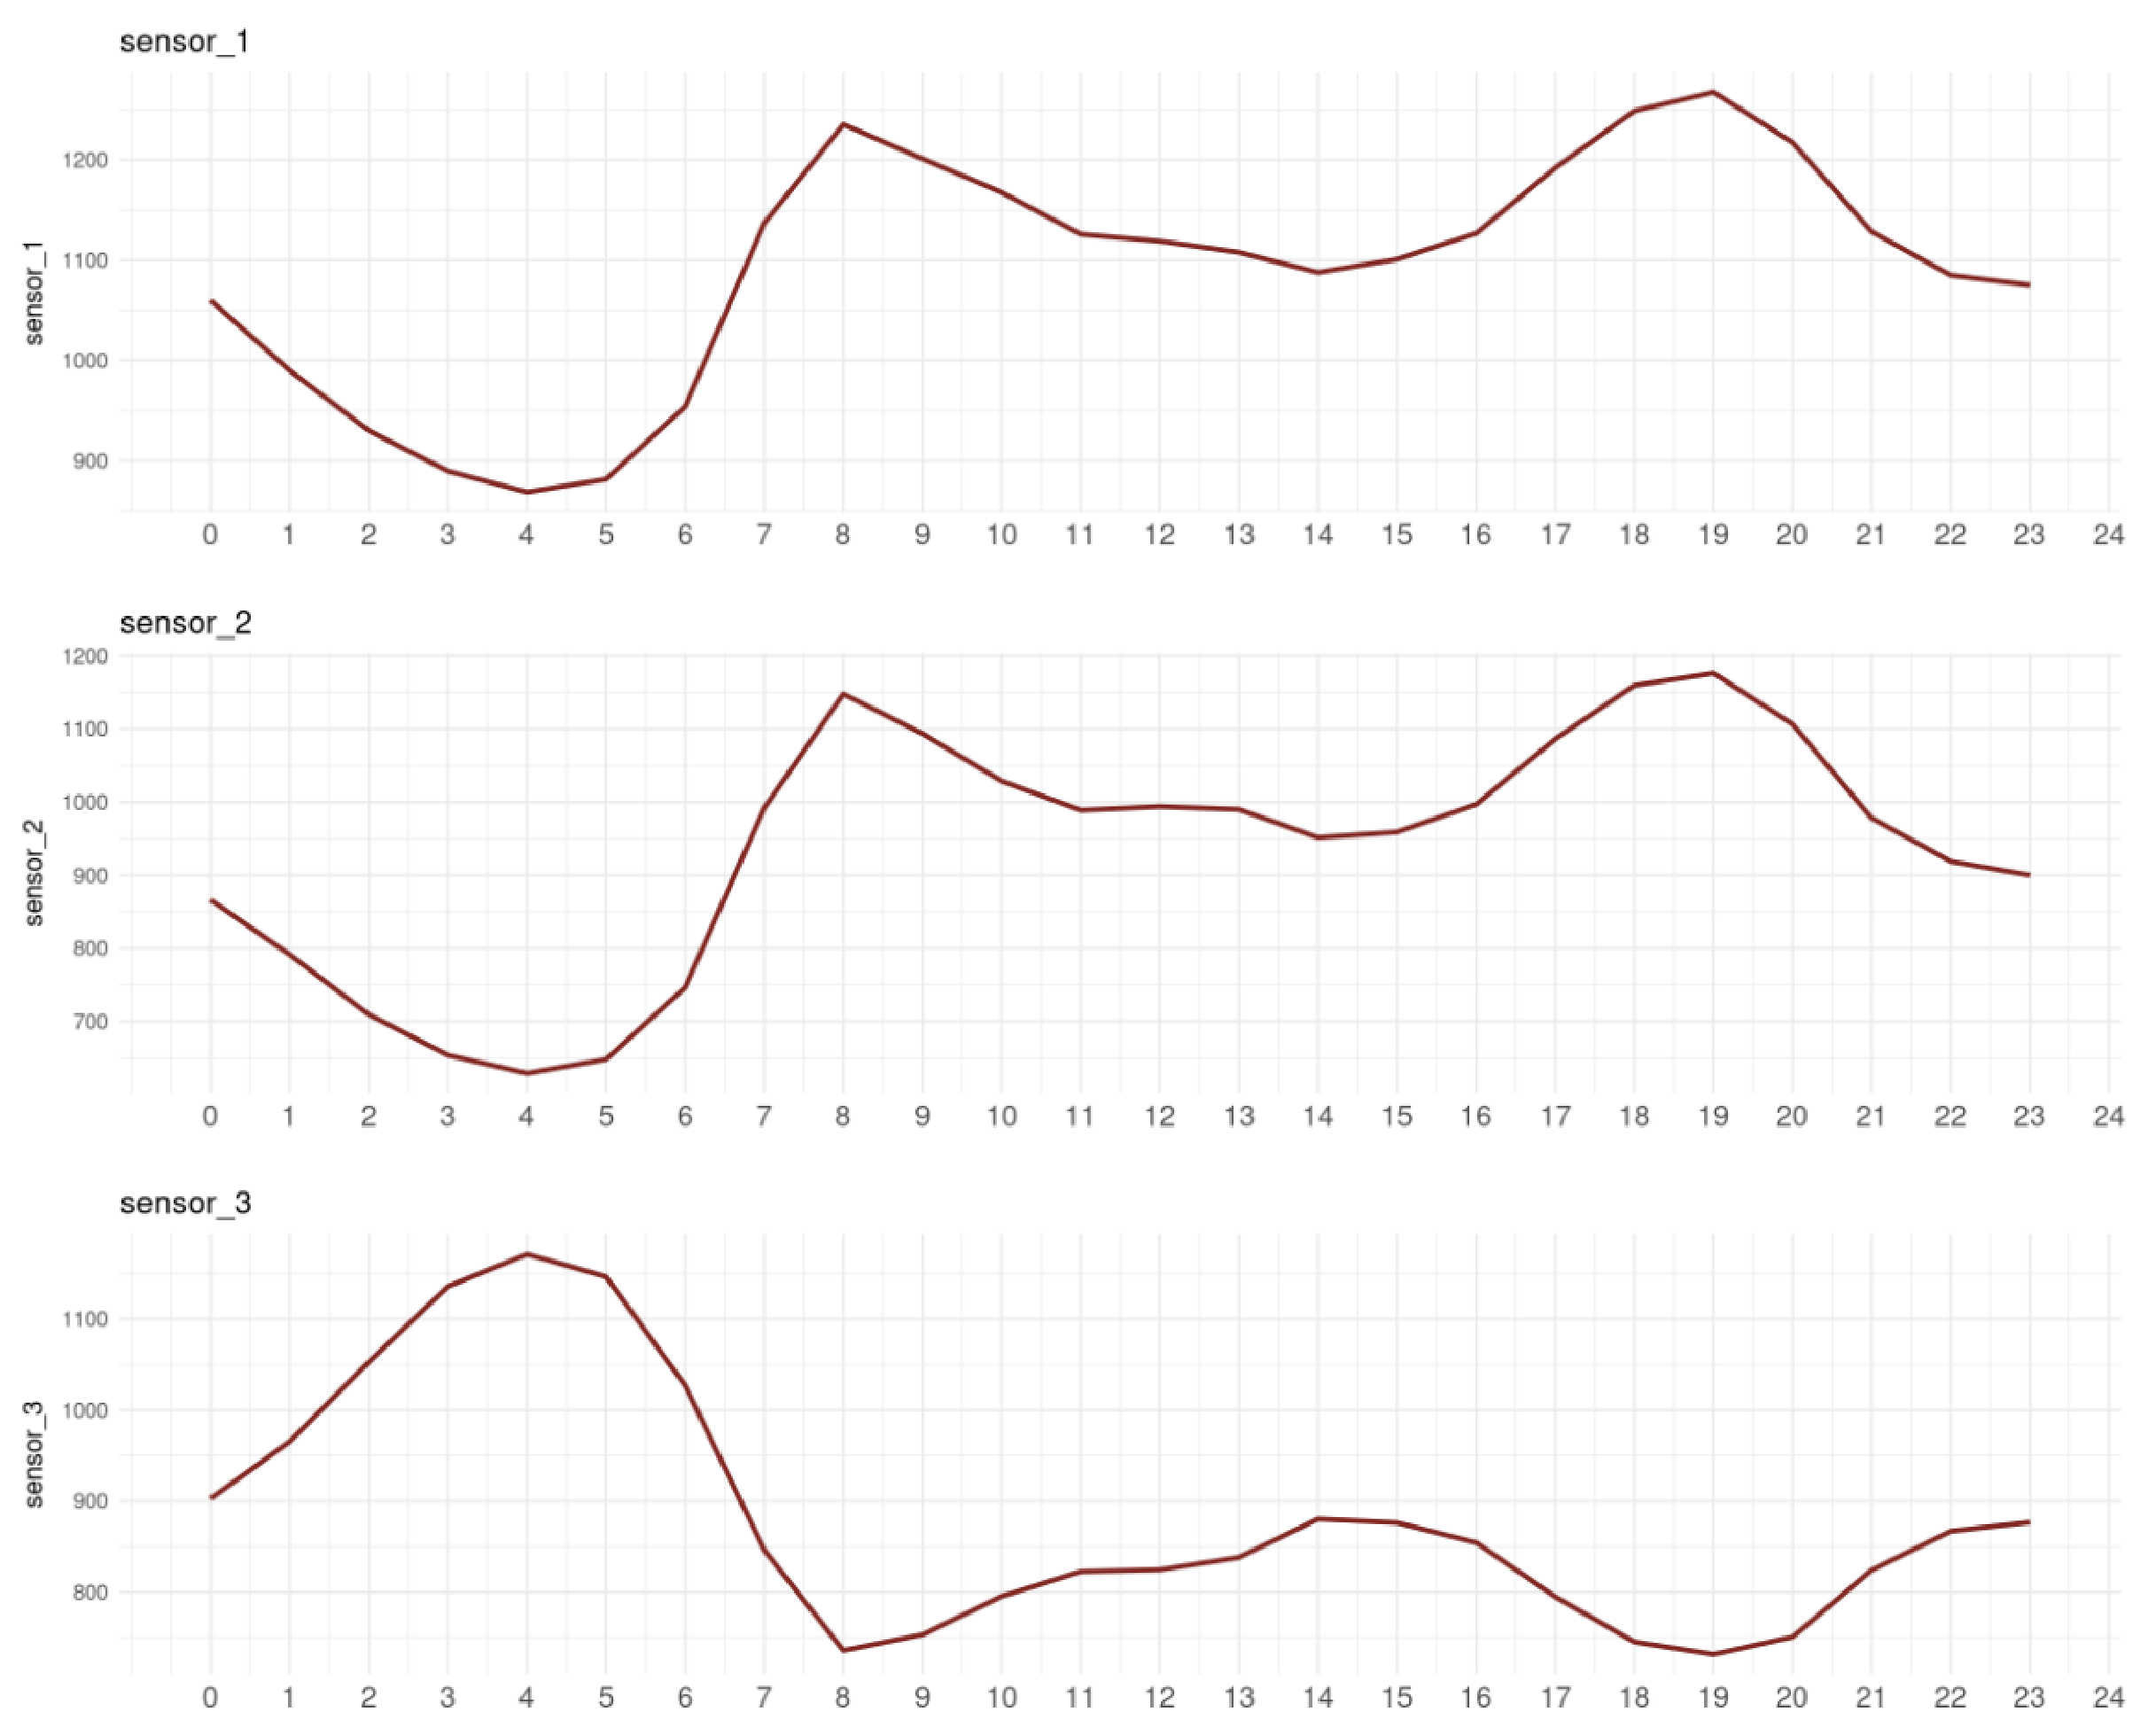
\includegraphics[scale=0.3]{figures//p6.eps}\\
		\caption{Sensor(1-3) Daily Hourly Change}\label{fig:Sensor(1-3) Daily Hourly Change}
	\end{figure}
	
\end{slide}
%%
%%==========================================================================================

%%==========================================================================================
%%
\begin{slide}[toc=,bm=]{Data Visualization(7)}
	
	\begin{figure}
		\centering
		\selectcolormodel{rgb}
        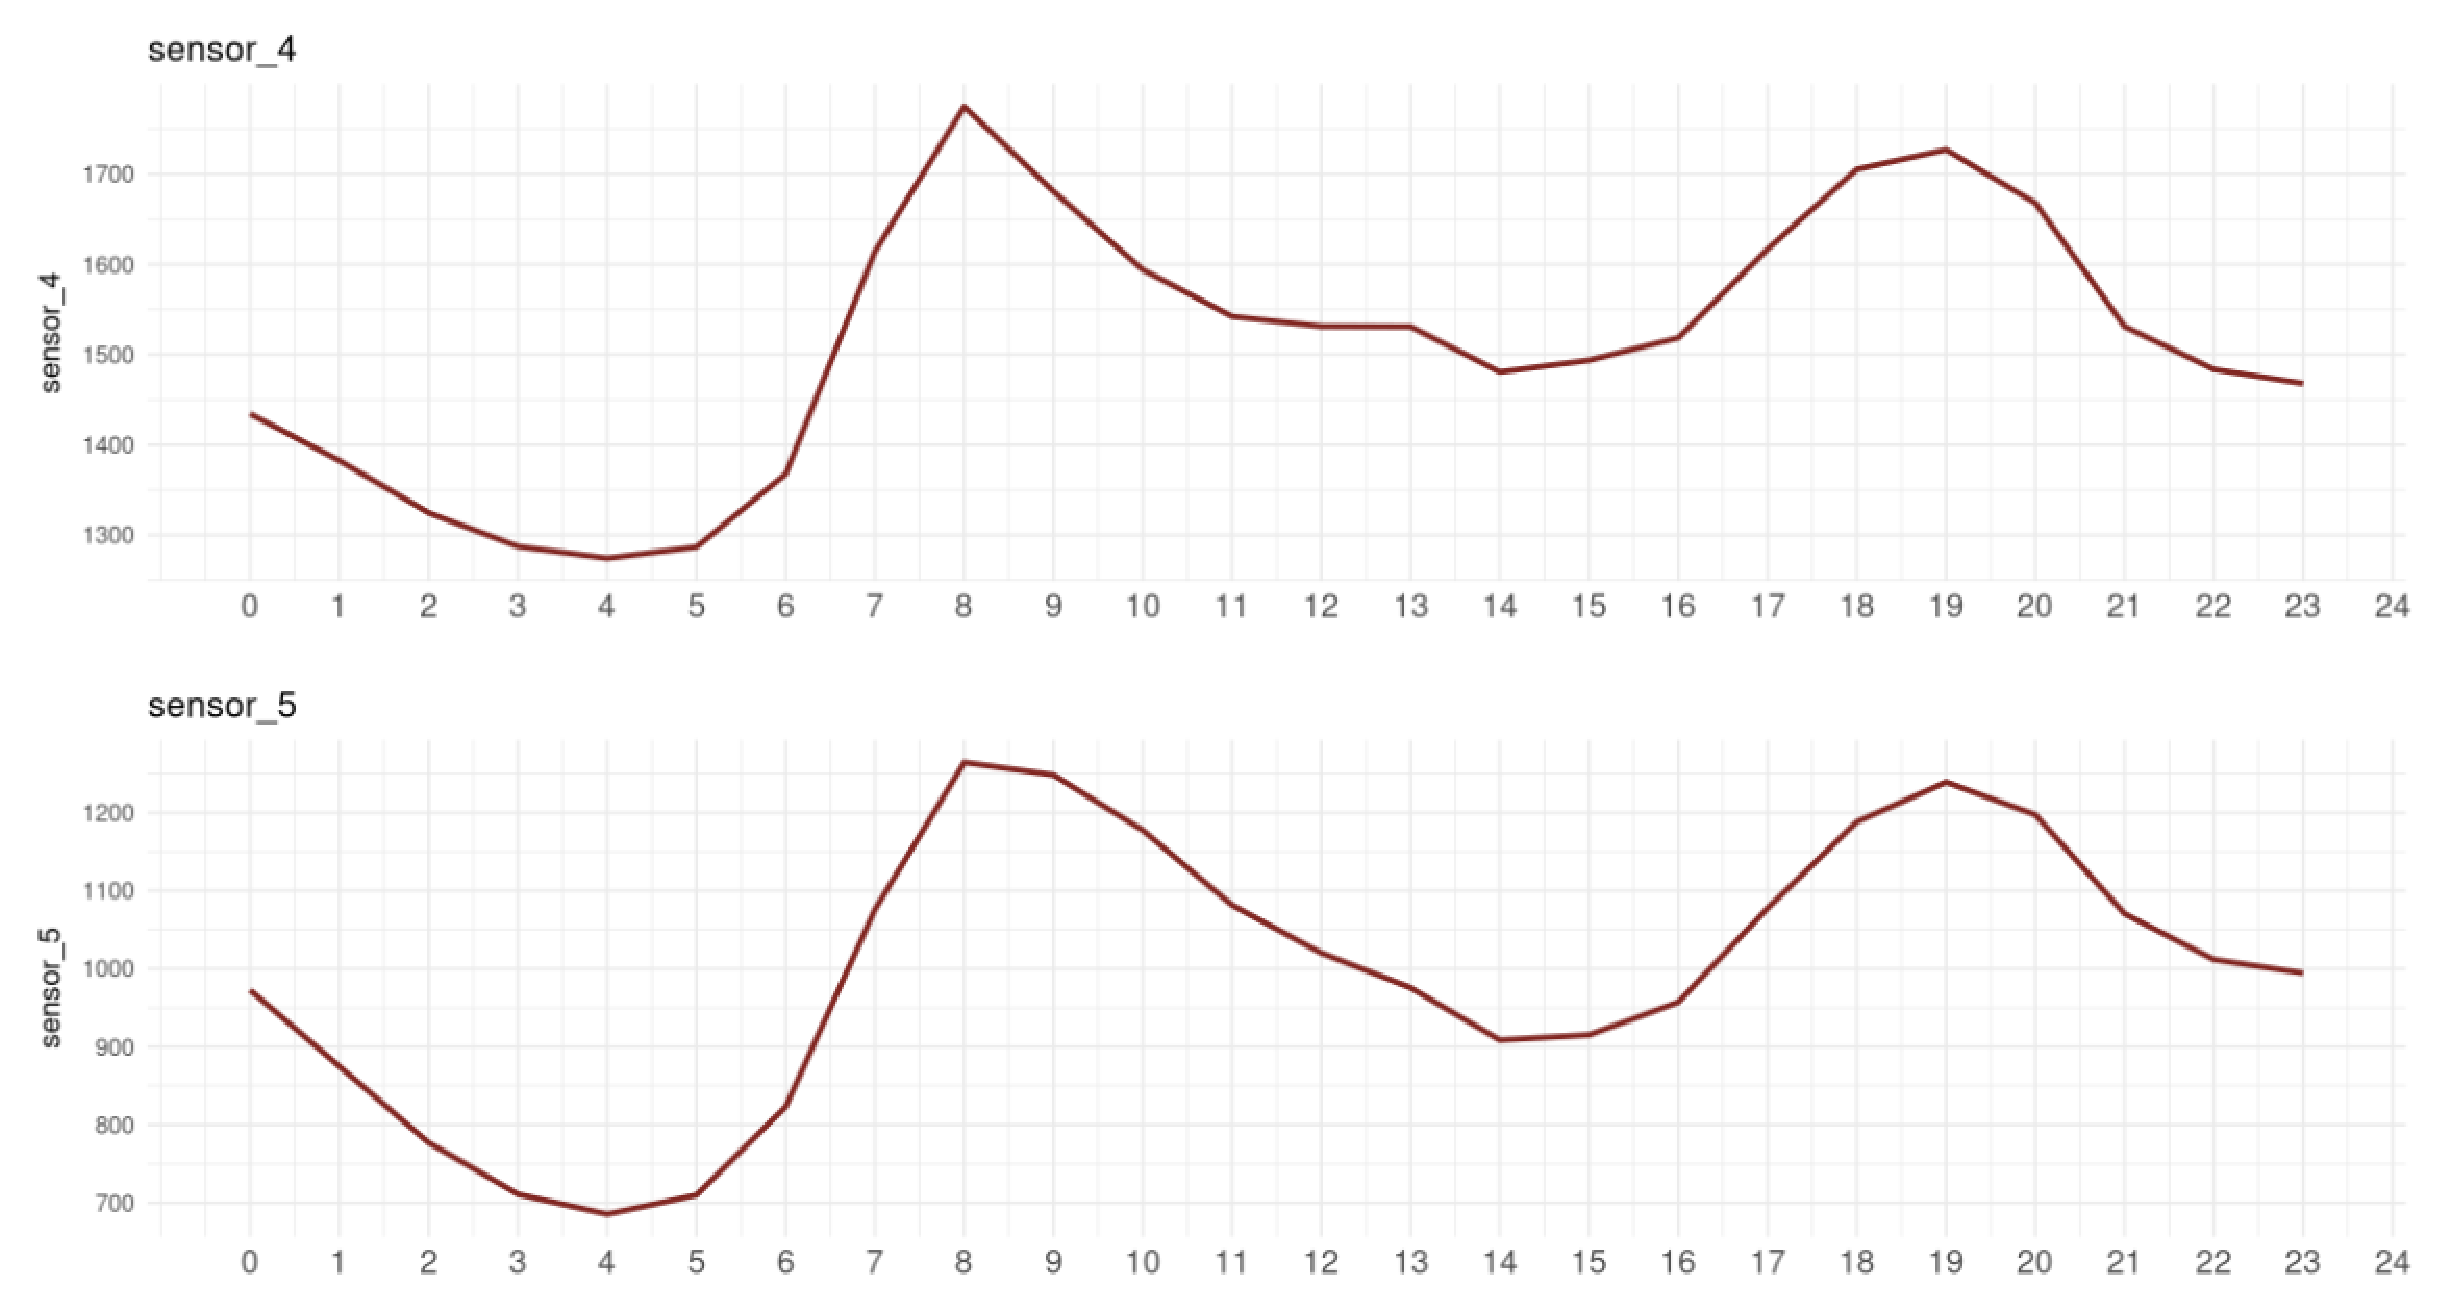
\includegraphics[scale=0.35]{figures//p7.eps}\\
		\caption{Sensor(4-5) Daily Hourly Change}\label{fig:Sensor(4-5) Daily Hourly Change}
	\end{figure}
	
\end{slide}
%%
%%==========================================================================================

%%==========================================================================================
%%
\begin{slide}[toc=,bm=]{Data Visualization(8)}
	
	\begin{figure}
		\centering
		\selectcolormodel{rgb}
		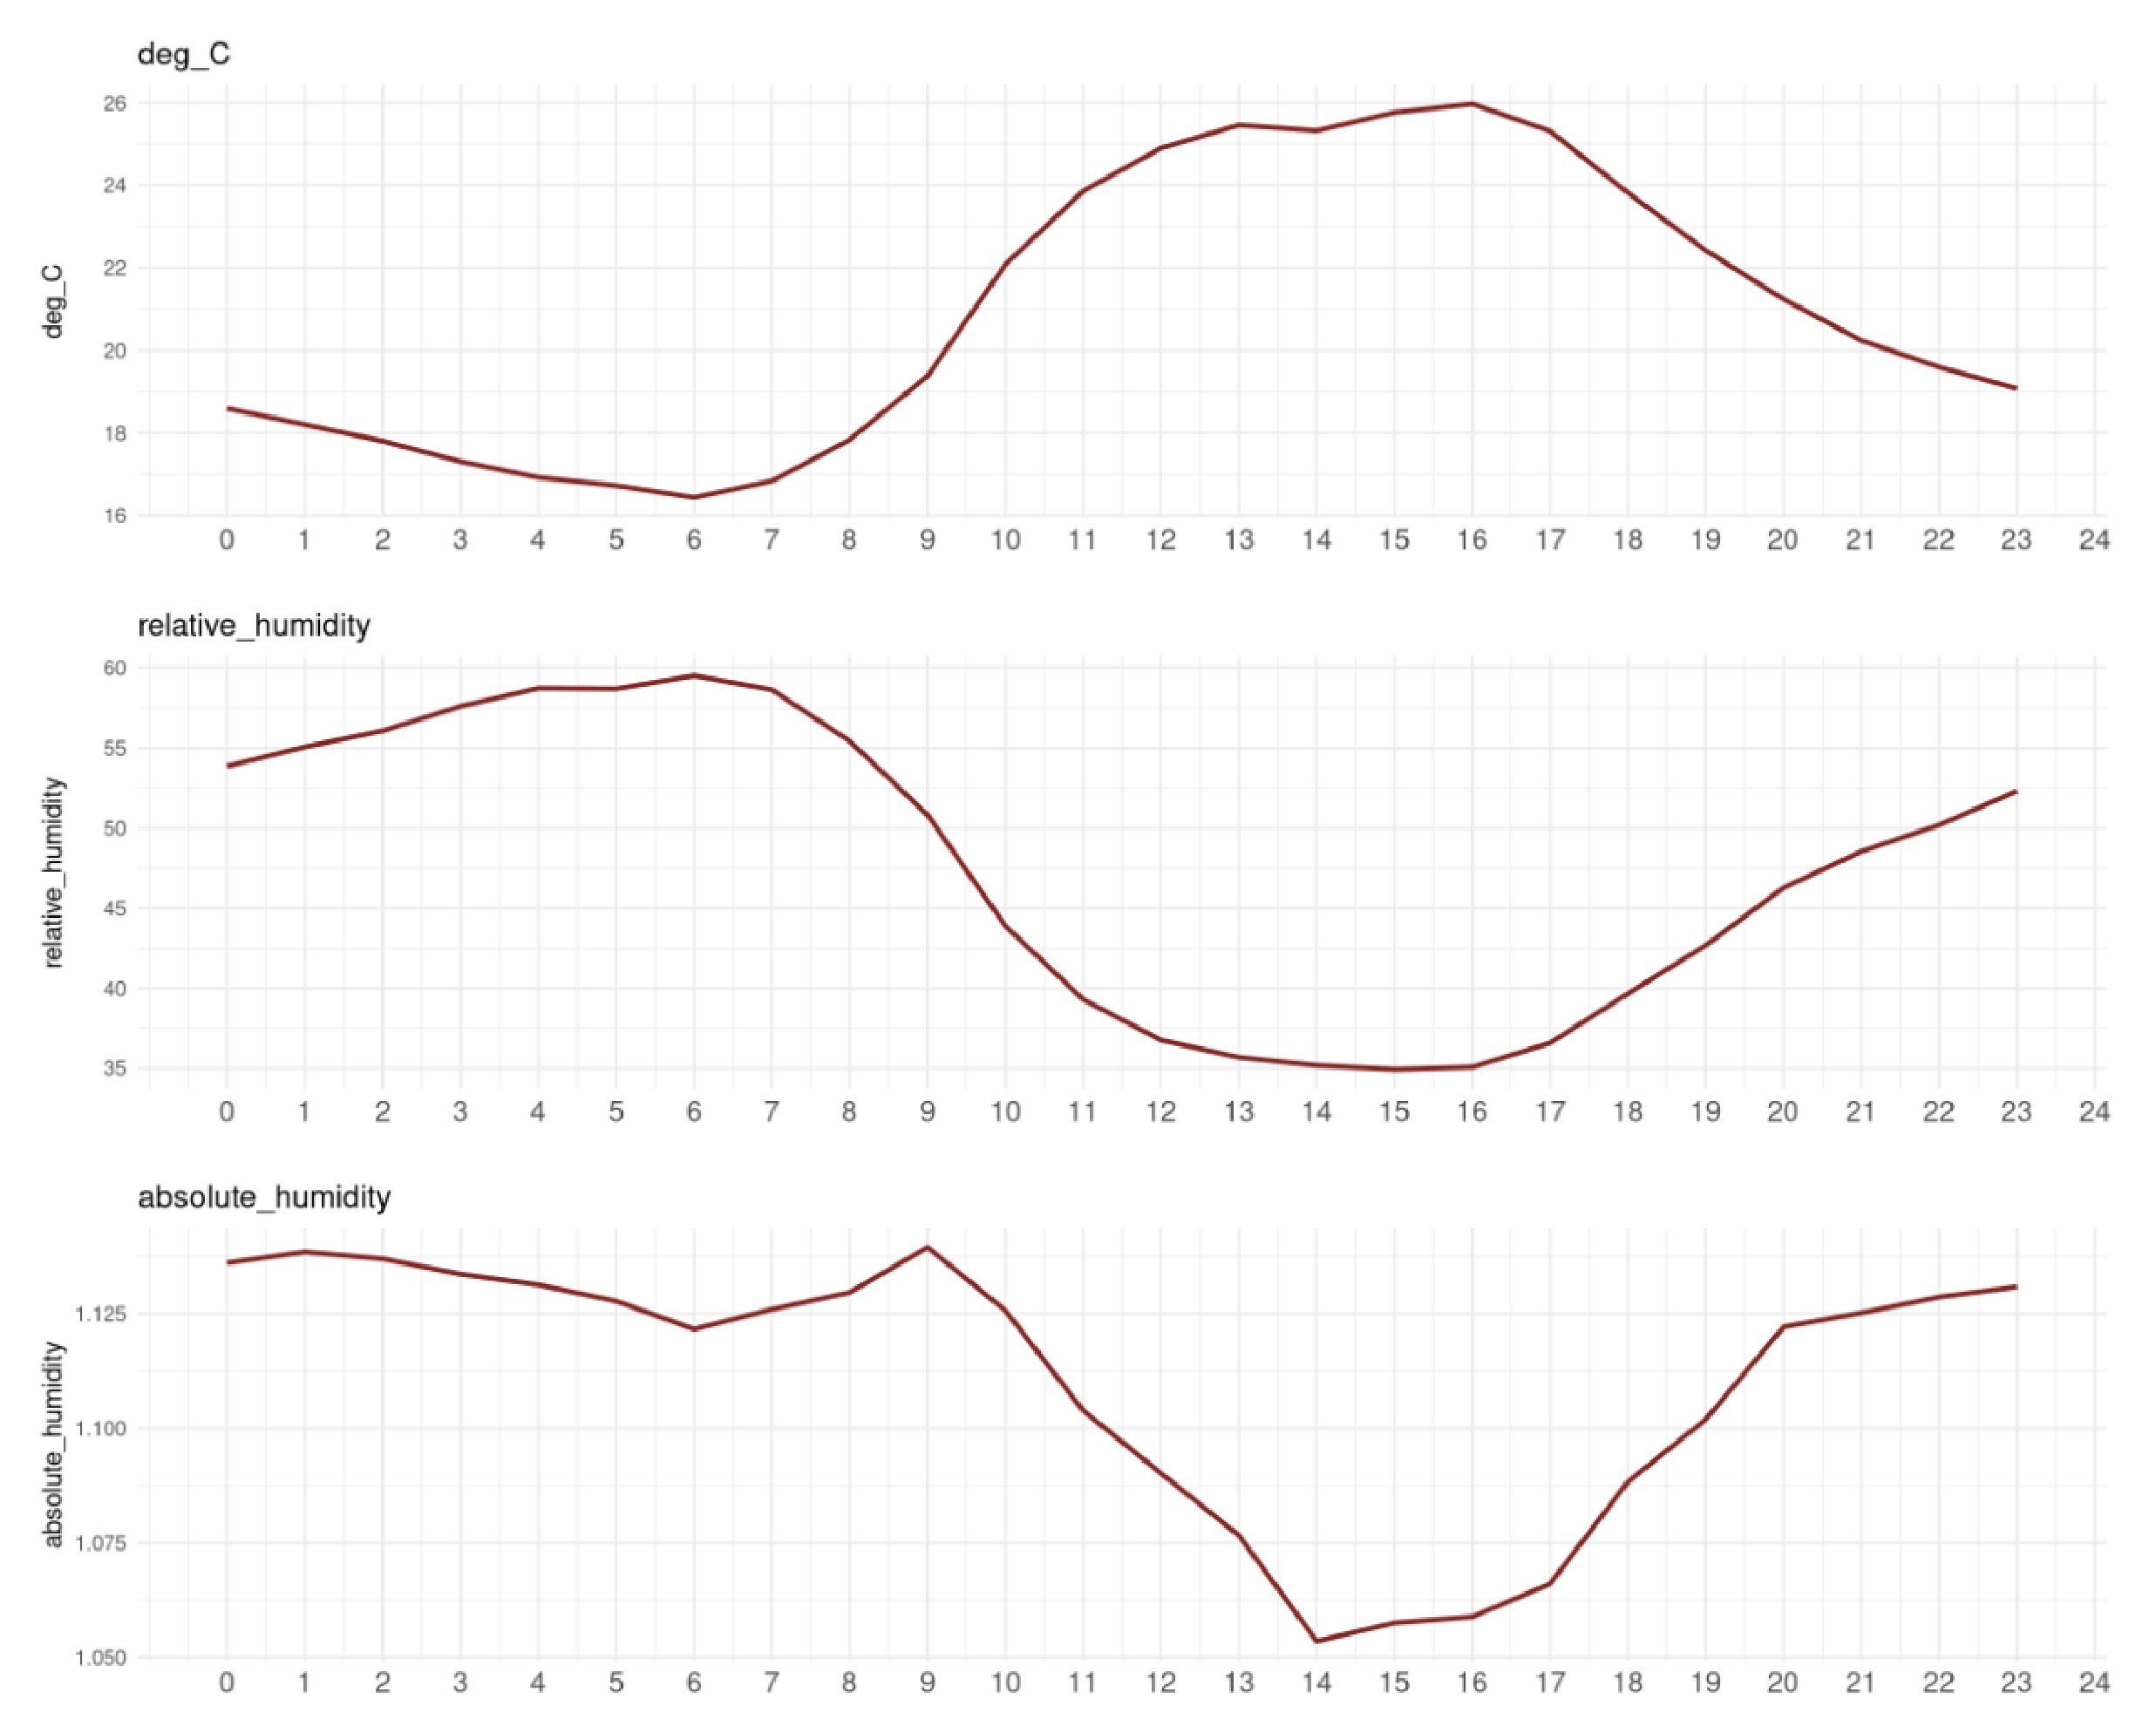
\includegraphics[scale=0.3]{figures//p8.eps}\\
		\caption{Weather Daily Hourly Change}\label{fig:Weather Daily Hourly Change}
	\end{figure}
	
\end{slide}
%%
%%==========================================================================================

%%==========================================================================================
%%
\begin{slide}[toc=,bm=]{Data Visualization(9)}
	
	\begin{figure}
		\centering
		\selectcolormodel{rgb}
		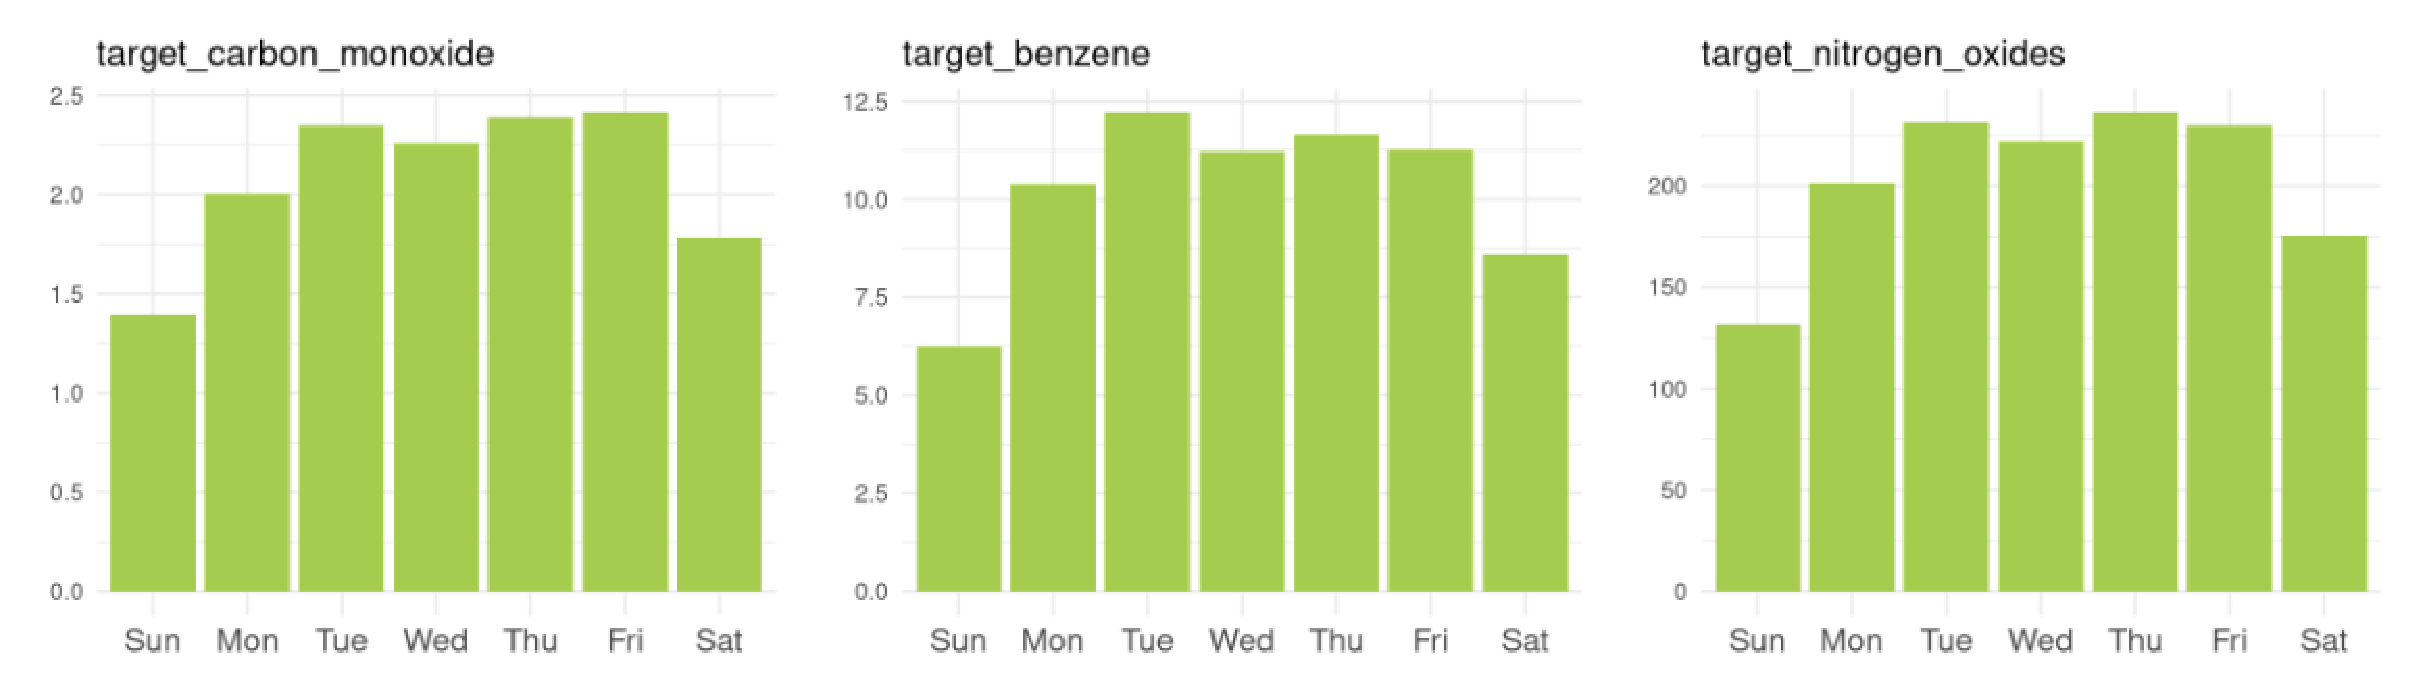
\includegraphics[scale=0.45]{figures//p9.eps}\\
		\caption{Target Weekly Situation}\label{fig:Target Weekly Situation}
	\end{figure}
	
\end{slide}
%%
%%==========================================================================================

%%==========================================================================================
%%
\begin{slide}[toc=,bm=]{Data Visualization(10)}
	
	\begin{figure}
		\centering
		\selectcolormodel{rgb}
		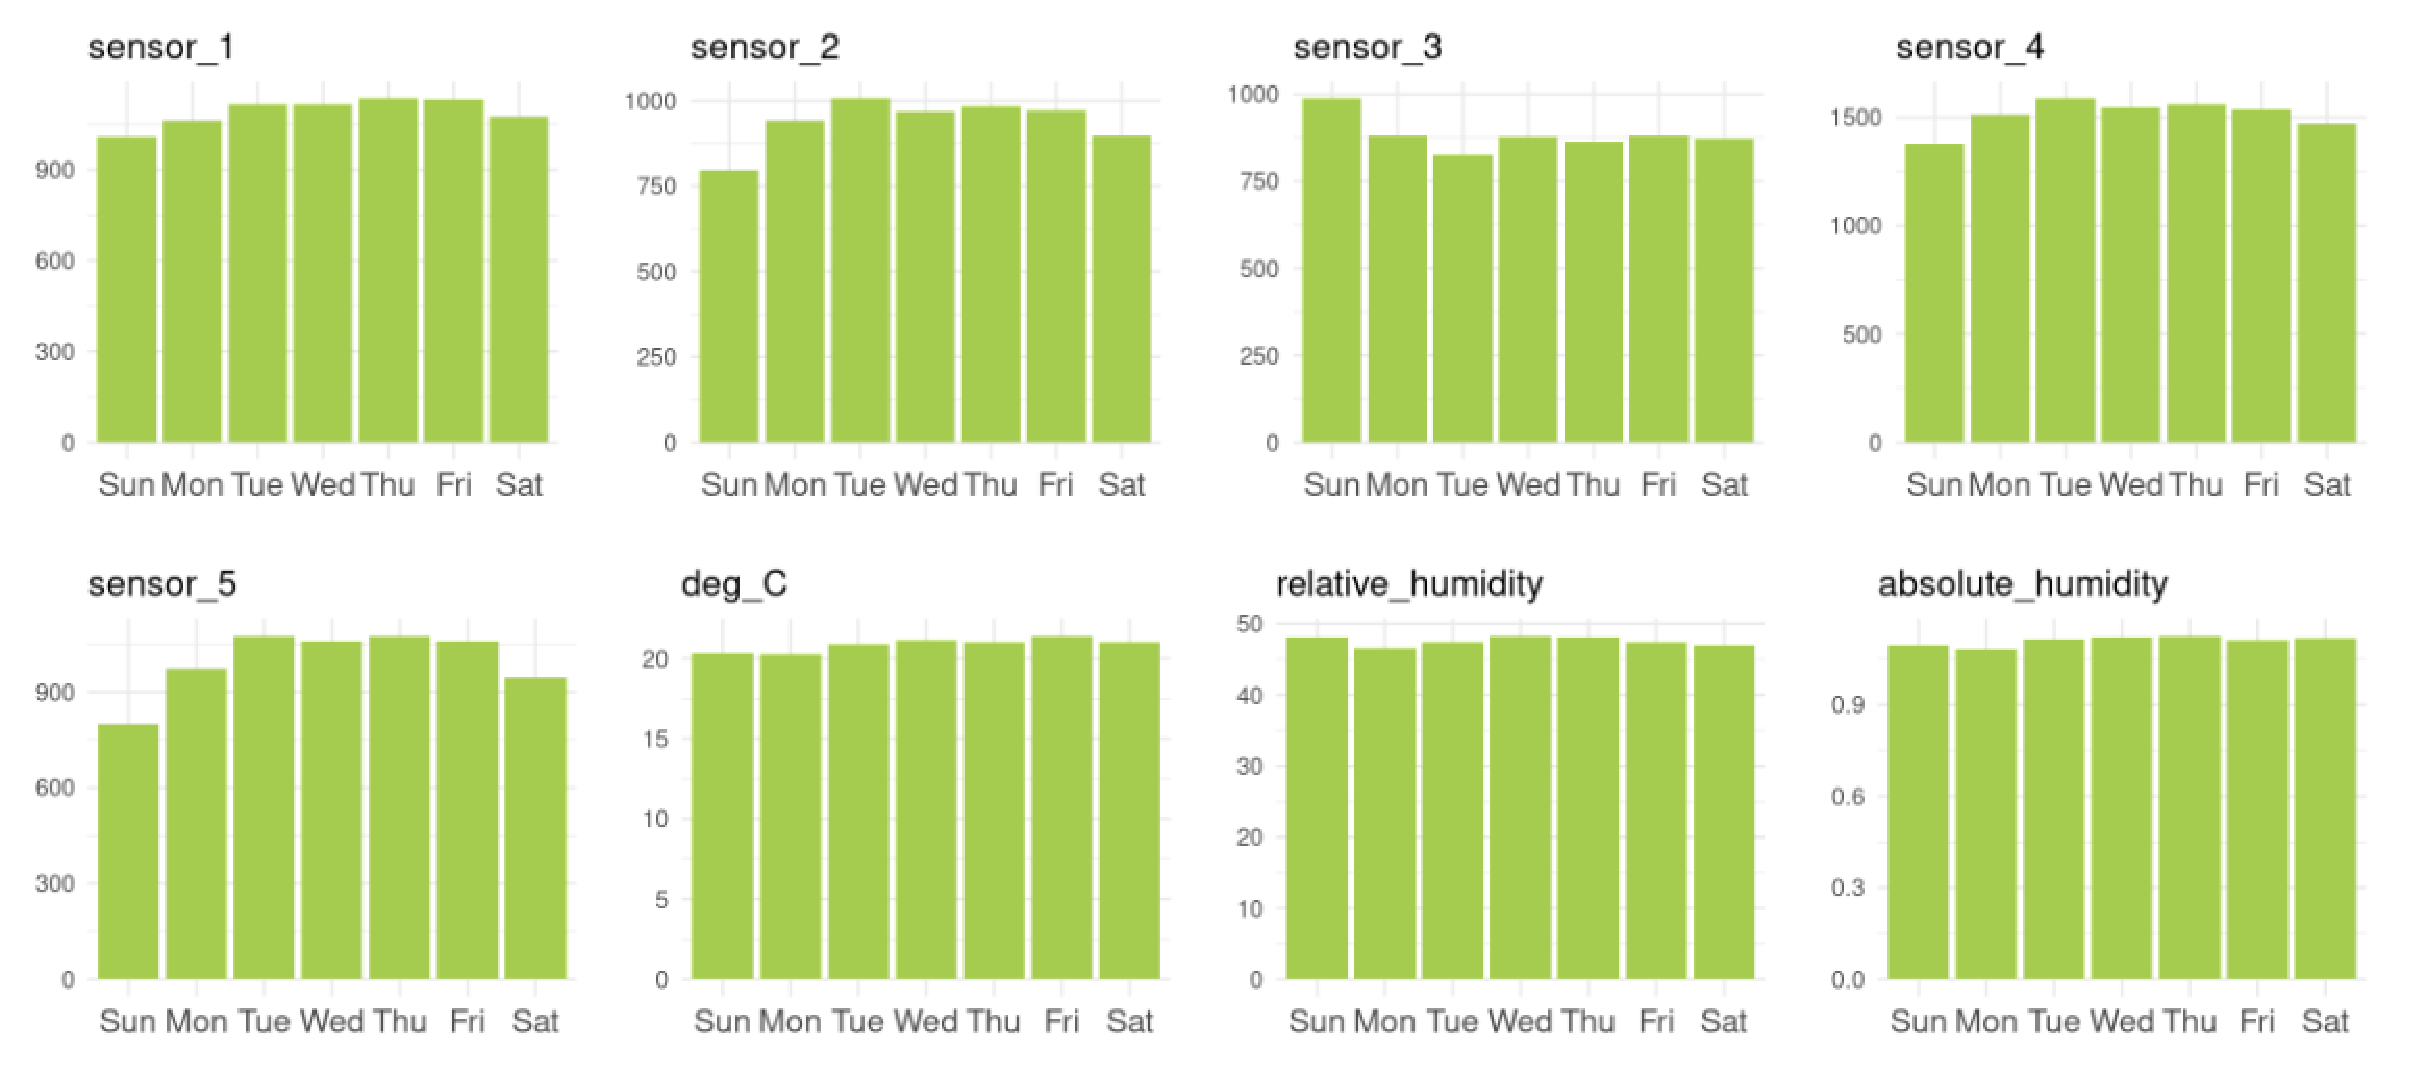
\includegraphics[scale=0.45]{figures//p10.eps}\\
		\caption{Sensor and Weather Weekly Situation}\label{fig:Sensor and Weather Weekly Situation}
	\end{figure}
	
\end{slide}
%%
%%==========================================================================================

%%==========================================================================================
%%



\section{Feature Engineering}
%%==========================================================================================
%%
\begin{slide}[toc=,bm=]{Feature Selection}
\begin{center}
	\twotonebox{\rotatebox{90}{}}{\parbox{.86\textwidth}
		{According to the analysis of training data, the following features are used for model training:
			\begin{itemize}
				\item absolute_humidity
				\item deg_C
				\item relative_humidity
				\item sensor1-5
				\item month
				\item week
				\item is_weekend
				\item hour
			\end{itemize}
	}}
\end{center}
\end{slide}
%%
%%==========================================================================================


\section{Model Training}
%%==========================================================================================
%%
\begin{slide}[toc=,bm=]{Model Selection}
\begin{center}
	\twotonebox{\rotatebox{90}{}}{\parbox{.86\textwidth}
		{Data fitting using LGBMRegressor, the algorithm is easy to use. 
			It only needs to put the set features and three prediction targets into the model for training, 
			but there is no parameter optimization, which has a certain impact on the training results.
	}}
\end{center}
\end{slide}
%%
%%==========================================================================================



\section{Result}

%%==========================================================================================
%%
\begin{slide}[toc=,bm=]{Result}
\begin{itemize}
\item
\smallskip
Use RMSLE(Root Mean Squared Logarithmic Error) to evaluate the results.
\begin{figure}
	\centering
	\selectcolormodel{rgb}
	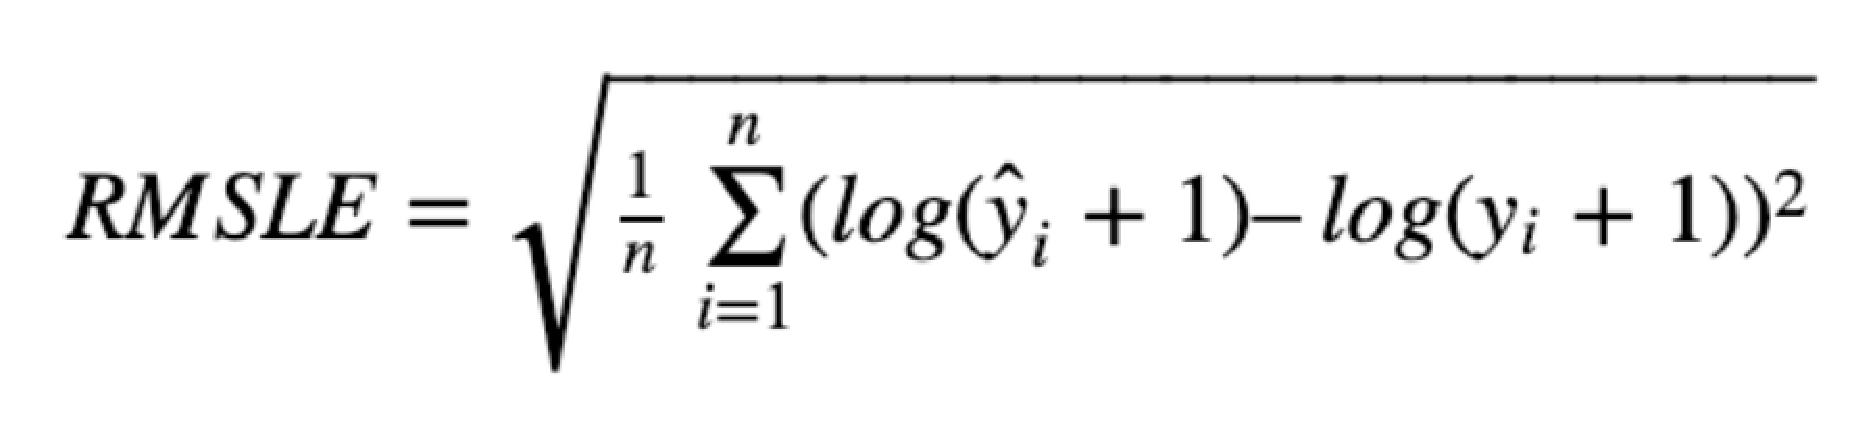
\includegraphics[scale=0.3]{figures//RMSLE.eps}\\
\end{figure}


\item
\smallskip
Private Score:0.33979

\item
\smallskip
Public Score:0.387

\end{itemize}
\end{slide}
%%
%%==========================================================================================


%%==========================================================================================
%
\begin{slide}[toc=,bm=]{Questions?}
\begin{center}
\begin{figure}
    \animategraphics[autoplay, loop, height=0.4\textheight]{5}{./graphics//gif//question//q_}{1}{30}
\end{figure}
\end{center}
\end{slide}
%%
%%==========================================================================================


%%==========================================================================================
% TODO: Contact Page
\begin{wideslide}[toc=,bm=]{Contact Information}
\centering
\vspace{\stretch{1}}
\twocolumn[
lcolwidth=0.35\linewidth,
rcolwidth=0.65\linewidth
]
{
% \centerline{
\includegraphics[scale=.2]{tulip-logo.eps}}
}
{
\vspace{\stretch{1}}
Yu Li\\
School of Economics and Management\\
Nanjing University of Science and Technology, China
\begin{description}
 \item[\textcolor{orange}{\faEnvelope}] \href{mailto:2805242929@qq.com}
 {\textsc{\footnotesize{2805242929@qq.com}}}

 \item[\textcolor{orange}{\faHome}] \href{http://www.tulip.org.au}
 {\textsc{\footnotesize{Team for Universal Learning and Intelligent Processing}}}
\end{description}
}
\vspace{\stretch{1}}
\end{wideslide}

\end{document}

\endinput
